% Options for packages loaded elsewhere
\PassOptionsToPackage{unicode}{hyperref}
\PassOptionsToPackage{hyphens}{url}
\PassOptionsToPackage{dvipsnames,svgnames,x11names}{xcolor}
%
\documentclass[
  a4paper,
]{article}

\usepackage{amsmath,amssymb}
\usepackage{iftex}
\ifPDFTeX
  \usepackage[T1]{fontenc}
  \usepackage[utf8]{inputenc}
  \usepackage{textcomp} % provide euro and other symbols
\else % if luatex or xetex
  \usepackage{unicode-math}
  \defaultfontfeatures{Scale=MatchLowercase}
  \defaultfontfeatures[\rmfamily]{Ligatures=TeX,Scale=1}
\fi
\usepackage{lmodern}
\ifPDFTeX\else  
    % xetex/luatex font selection
\fi
% Use upquote if available, for straight quotes in verbatim environments
\IfFileExists{upquote.sty}{\usepackage{upquote}}{}
\IfFileExists{microtype.sty}{% use microtype if available
  \usepackage[]{microtype}
  \UseMicrotypeSet[protrusion]{basicmath} % disable protrusion for tt fonts
}{}
\makeatletter
\@ifundefined{KOMAClassName}{% if non-KOMA class
  \IfFileExists{parskip.sty}{%
    \usepackage{parskip}
  }{% else
    \setlength{\parindent}{0pt}
    \setlength{\parskip}{6pt plus 2pt minus 1pt}}
}{% if KOMA class
  \KOMAoptions{parskip=half}}
\makeatother
\usepackage{xcolor}
\usepackage[top=2.54cm,right=2.54cm,bottom=2.54cm,left=2.54cm]{geometry}
\setlength{\emergencystretch}{3em} % prevent overfull lines
\setcounter{secnumdepth}{-\maxdimen} % remove section numbering
% Make \paragraph and \subparagraph free-standing
\ifx\paragraph\undefined\else
  \let\oldparagraph\paragraph
  \renewcommand{\paragraph}[1]{\oldparagraph{#1}\mbox{}}
\fi
\ifx\subparagraph\undefined\else
  \let\oldsubparagraph\subparagraph
  \renewcommand{\subparagraph}[1]{\oldsubparagraph{#1}\mbox{}}
\fi

\usepackage{color}
\usepackage{fancyvrb}
\newcommand{\VerbBar}{|}
\newcommand{\VERB}{\Verb[commandchars=\\\{\}]}
\DefineVerbatimEnvironment{Highlighting}{Verbatim}{commandchars=\\\{\}}
% Add ',fontsize=\small' for more characters per line
\newenvironment{Shaded}{}{}
\newcommand{\AlertTok}[1]{\textcolor[rgb]{1.00,0.33,0.33}{\textbf{#1}}}
\newcommand{\AnnotationTok}[1]{\textcolor[rgb]{0.42,0.45,0.49}{#1}}
\newcommand{\AttributeTok}[1]{\textcolor[rgb]{0.84,0.23,0.29}{#1}}
\newcommand{\BaseNTok}[1]{\textcolor[rgb]{0.00,0.36,0.77}{#1}}
\newcommand{\BuiltInTok}[1]{\textcolor[rgb]{0.84,0.23,0.29}{#1}}
\newcommand{\CharTok}[1]{\textcolor[rgb]{0.01,0.18,0.38}{#1}}
\newcommand{\CommentTok}[1]{\textcolor[rgb]{0.42,0.45,0.49}{#1}}
\newcommand{\CommentVarTok}[1]{\textcolor[rgb]{0.42,0.45,0.49}{#1}}
\newcommand{\ConstantTok}[1]{\textcolor[rgb]{0.00,0.36,0.77}{#1}}
\newcommand{\ControlFlowTok}[1]{\textcolor[rgb]{0.84,0.23,0.29}{#1}}
\newcommand{\DataTypeTok}[1]{\textcolor[rgb]{0.84,0.23,0.29}{#1}}
\newcommand{\DecValTok}[1]{\textcolor[rgb]{0.00,0.36,0.77}{#1}}
\newcommand{\DocumentationTok}[1]{\textcolor[rgb]{0.42,0.45,0.49}{#1}}
\newcommand{\ErrorTok}[1]{\textcolor[rgb]{1.00,0.33,0.33}{\underline{#1}}}
\newcommand{\ExtensionTok}[1]{\textcolor[rgb]{0.84,0.23,0.29}{\textbf{#1}}}
\newcommand{\FloatTok}[1]{\textcolor[rgb]{0.00,0.36,0.77}{#1}}
\newcommand{\FunctionTok}[1]{\textcolor[rgb]{0.44,0.26,0.76}{#1}}
\newcommand{\ImportTok}[1]{\textcolor[rgb]{0.01,0.18,0.38}{#1}}
\newcommand{\InformationTok}[1]{\textcolor[rgb]{0.42,0.45,0.49}{#1}}
\newcommand{\KeywordTok}[1]{\textcolor[rgb]{0.84,0.23,0.29}{#1}}
\newcommand{\NormalTok}[1]{\textcolor[rgb]{0.14,0.16,0.18}{#1}}
\newcommand{\OperatorTok}[1]{\textcolor[rgb]{0.14,0.16,0.18}{#1}}
\newcommand{\OtherTok}[1]{\textcolor[rgb]{0.44,0.26,0.76}{#1}}
\newcommand{\PreprocessorTok}[1]{\textcolor[rgb]{0.84,0.23,0.29}{#1}}
\newcommand{\RegionMarkerTok}[1]{\textcolor[rgb]{0.42,0.45,0.49}{#1}}
\newcommand{\SpecialCharTok}[1]{\textcolor[rgb]{0.00,0.36,0.77}{#1}}
\newcommand{\SpecialStringTok}[1]{\textcolor[rgb]{0.01,0.18,0.38}{#1}}
\newcommand{\StringTok}[1]{\textcolor[rgb]{0.01,0.18,0.38}{#1}}
\newcommand{\VariableTok}[1]{\textcolor[rgb]{0.89,0.38,0.04}{#1}}
\newcommand{\VerbatimStringTok}[1]{\textcolor[rgb]{0.01,0.18,0.38}{#1}}
\newcommand{\WarningTok}[1]{\textcolor[rgb]{1.00,0.33,0.33}{#1}}

\providecommand{\tightlist}{%
  \setlength{\itemsep}{0pt}\setlength{\parskip}{0pt}}\usepackage{longtable,booktabs,array}
\usepackage{calc} % for calculating minipage widths
% Correct order of tables after \paragraph or \subparagraph
\usepackage{etoolbox}
\makeatletter
\patchcmd\longtable{\par}{\if@noskipsec\mbox{}\fi\par}{}{}
\makeatother
% Allow footnotes in longtable head/foot
\IfFileExists{footnotehyper.sty}{\usepackage{footnotehyper}}{\usepackage{footnote}}
\makesavenoteenv{longtable}
\usepackage{graphicx}
\makeatletter
\def\maxwidth{\ifdim\Gin@nat@width>\linewidth\linewidth\else\Gin@nat@width\fi}
\def\maxheight{\ifdim\Gin@nat@height>\textheight\textheight\else\Gin@nat@height\fi}
\makeatother
% Scale images if necessary, so that they will not overflow the page
% margins by default, and it is still possible to overwrite the defaults
% using explicit options in \includegraphics[width, height, ...]{}
\setkeys{Gin}{width=\maxwidth,height=\maxheight,keepaspectratio}
% Set default figure placement to htbp
\makeatletter
\def\fps@figure{htbp}
\makeatother

\makeatletter
\makeatother
\makeatletter
\makeatother
\makeatletter
\@ifpackageloaded{caption}{}{\usepackage{caption}}
\AtBeginDocument{%
\ifdefined\contentsname
  \renewcommand*\contentsname{Tabla de contenidos}
\else
  \newcommand\contentsname{Tabla de contenidos}
\fi
\ifdefined\listfigurename
  \renewcommand*\listfigurename{Listado de Figuras}
\else
  \newcommand\listfigurename{Listado de Figuras}
\fi
\ifdefined\listtablename
  \renewcommand*\listtablename{Listado de Tablas}
\else
  \newcommand\listtablename{Listado de Tablas}
\fi
\ifdefined\figurename
  \renewcommand*\figurename{Figura}
\else
  \newcommand\figurename{Figura}
\fi
\ifdefined\tablename
  \renewcommand*\tablename{Tabla}
\else
  \newcommand\tablename{Tabla}
\fi
}
\@ifpackageloaded{float}{}{\usepackage{float}}
\floatstyle{ruled}
\@ifundefined{c@chapter}{\newfloat{codelisting}{h}{lop}}{\newfloat{codelisting}{h}{lop}[chapter]}
\floatname{codelisting}{Listado}
\newcommand*\listoflistings{\listof{codelisting}{Listado de Listados}}
\makeatother
\makeatletter
\@ifpackageloaded{caption}{}{\usepackage{caption}}
\@ifpackageloaded{subcaption}{}{\usepackage{subcaption}}
\makeatother
\makeatletter
\@ifpackageloaded{tcolorbox}{}{\usepackage[skins,breakable]{tcolorbox}}
\makeatother
\makeatletter
\@ifundefined{shadecolor}{\definecolor{shadecolor}{rgb}{.97, .97, .97}}
\makeatother
\makeatletter
\makeatother
\makeatletter
\makeatother
\ifLuaTeX
\usepackage[bidi=basic]{babel}
\else
\usepackage[bidi=default]{babel}
\fi
\babelprovide[main,import]{spanish}
% get rid of language-specific shorthands (see #6817):
\let\LanguageShortHands\languageshorthands
\def\languageshorthands#1{}
\ifLuaTeX
  \usepackage{selnolig}  % disable illegal ligatures
\fi
\usepackage[]{biblatex}
\addbibresource{../../../../references.bib}
\IfFileExists{bookmark.sty}{\usepackage{bookmark}}{\usepackage{hyperref}}
\IfFileExists{xurl.sty}{\usepackage{xurl}}{} % add URL line breaks if available
\urlstyle{same} % disable monospaced font for URLs
\hypersetup{
  pdftitle={Graficos con python},
  pdfauthor={Edison Achalma},
  pdflang={es},
  colorlinks=true,
  linkcolor={blue},
  filecolor={Maroon},
  citecolor={Blue},
  urlcolor={Blue},
  pdfcreator={LaTeX via pandoc}}

\title{Graficos con python}
\usepackage{etoolbox}
\makeatletter
\providecommand{\subtitle}[1]{% add subtitle to \maketitle
  \apptocmd{\@title}{\par {\large #1 \par}}{}{}
}
\makeatother
\subtitle{E}
\author{Edison Achalma}
\date{2023-06-23}

\begin{document}
\maketitle
\ifdefined\Shaded\renewenvironment{Shaded}{\begin{tcolorbox}[sharp corners, interior hidden, frame hidden, breakable, enhanced, borderline west={3pt}{0pt}{shadecolor}, boxrule=0pt]}{\end{tcolorbox}}\fi

\hypertarget{introducciuxf3n-a-los-gruxe1ficos-con-python}{%
\section{Introducción a los gráficos con
Python}\label{introducciuxf3n-a-los-gruxe1ficos-con-python}}

\hypertarget{por-quuxe9-los-gruxe1ficos-son-importantes-en-el-anuxe1lisis-de-datos}{%
\subsection{¿Por qué los gráficos son importantes en el análisis de
datos?}\label{por-quuxe9-los-gruxe1ficos-son-importantes-en-el-anuxe1lisis-de-datos}}

Cuando nos enfrentamos a un conjunto de datos, a veces puede resultar
abrumador tratar de extraer información significativa y comprender
patrones importantes. Aquí es donde entran en juego los gráficos. Los
gráficos son una herramienta visual poderosa que nos permite representar
datos de manera clara y comprensible.

Imagina esto: en lugar de mirar una larga lista de números o leer tablas
extensas, puedes ver tus datos plasmados en un gráfico colorido y fácil
de interpretar. Los gráficos nos permiten visualizar tendencias,
comparar valores y descubrir relaciones ocultas entre variables. Son
como una ventana que nos permite explorar y comprender los datos de
manera más intuitiva.

Los gráficos no solo hacen que el análisis de datos sea más accesible,
sino que también nos ayudan a comunicar nuestros hallazgos de manera
efectiva. Una imagen vale más que mil palabras, ¿verdad? Al presentar
información a través de gráficos, podemos transmitir mensajes complejos
de manera clara y concisa, lo que facilita que otras personas comprendan
nuestros resultados.

\hypertarget{ventajas-de-utilizar-python-para-crear-gruxe1ficos}{%
\subsection{Ventajas de utilizar Python para crear
gráficos}\label{ventajas-de-utilizar-python-para-crear-gruxe1ficos}}

Cuando se trata de crear gráficos, Python ofrece una serie de ventajas
que lo convierten en una herramienta popular y poderosa en el análisis
de datos. Veamos algunas de estas ventajas:

\begin{enumerate}
\def\labelenumi{\arabic{enumi}.}
\item
  \textbf{Facilidad de uso}: Python es un lenguaje de programación de
  alto nivel y fácil de aprender. Su sintaxis clara y legible permite a
  los usuarios escribir código de forma concisa y comprensible. Esto
  facilita la creación de gráficos, incluso para aquellos que no tienen
  experiencia previa en programación.
\item
  \textbf{Gran cantidad de bibliotecas}: Python cuenta con una amplia
  gama de bibliotecas especializadas en la visualización de datos.
  Algunas de las más populares son Matplotlib, Seaborn y Plotly. Estas
  bibliotecas ofrecen una variedad de estilos de gráficos, opciones de
  personalización y herramientas interactivas para explorar y presentar
  tus datos de manera efectiva.
\item
  \textbf{Compatibilidad con otras herramientas}: Python se integra
  fácilmente con otras herramientas y bibliotecas utilizadas en el
  análisis de datos. Puedes combinar el poder de Python con bibliotecas
  como Pandas para el procesamiento de datos, NumPy para operaciones
  numéricas y SciPy para análisis científico. Esta interoperabilidad
  facilita la manipulación y preparación de datos antes de crear tus
  gráficos.
\item
  \textbf{Comunidad activa}: Python cuenta con una gran comunidad de
  desarrolladores y usuarios que constantemente contribuyen con nuevas
  funcionalidades, mejoras y ejemplos de uso. Esto significa que siempre
  encontrarás recursos, tutoriales y soporte disponibles para ayudarte a
  resolver cualquier problema o desafío que encuentres al crear tus
  gráficos.
\item
  \textbf{Flexibilidad y versatilidad}: Python te permite crear una
  amplia variedad de gráficos, desde simples diagramas de barras hasta
  complejas visualizaciones en 3D. Puedes adaptar tus gráficos a tus
  necesidades específicas y personalizarlos con colores, etiquetas,
  leyendas y más. Además, puedes exportar tus gráficos en varios
  formatos de imagen o incrustarlos en informes y aplicaciones.
\end{enumerate}

\hypertarget{preparaciuxf3n-del-entorno-de-trabajo}{%
\section{Preparación del entorno de
trabajo}\label{preparaciuxf3n-del-entorno-de-trabajo}}

\hypertarget{instalaciuxf3n-de-python-y-las-bibliotecas-necesarias}{%
\subsection{Instalación de Python y las bibliotecas
necesarias}\label{instalaciuxf3n-de-python-y-las-bibliotecas-necesarias}}

Antes de sumergirnos en el emocionante mundo de los gráficos con Python,
es importante asegurarnos de tener todo configurado correctamente. A
continuación, te guiaré a través de los pasos para instalar Python y las
bibliotecas necesarias:

\textbf{Paso 1: Descargar Python} Dirígete al sitio web oficial de
Python (https://www.python.org/) y descarga la última versión estable.
Elige la versión adecuada para tu sistema operativo y sigue las
instrucciones de instalación.

\textbf{Paso 2: Verificar la instalación} Una vez que hayas instalado
Python, puedes verificar si se instaló correctamente abriendo una
ventana de terminal y escribiendo el siguiente comando:

\begin{verbatim}
python --version
\end{verbatim}

Si aparece la versión de Python que instalaste, ¡felicidades! Estás
listo para seguir adelante.

\textbf{Paso 3: Instalar las bibliotecas} Para crear gráficos con
Python, necesitarás instalar algunas bibliotecas populares como
Matplotlib, Seaborn y Plotly. Puedes instalar estas bibliotecas
utilizando el administrador de paquetes de Python, pip. Simplemente
ejecuta los siguientes comandos en tu terminal:

\begin{verbatim}
pip install matplotlib
pip install seaborn
pip install plotly
\end{verbatim}

Esto instalará las bibliotecas requeridas y todas sus dependencias.

¡Y eso es todo! Ahora tienes Python y las bibliotecas necesarias
instaladas en tu sistema. Estás listo para empezar a crear increíbles
gráficos y explorar tus datos de manera visual.

\hypertarget{configuraciuxf3n-del-entorno-de-desarrollo}{%
\subsection{Configuración del entorno de
desarrollo}\label{configuraciuxf3n-del-entorno-de-desarrollo}}

Antes de sumergirnos en la creación de gráficos increíbles, es
importante configurar nuestro entorno de desarrollo para trabajar de
manera eficiente. Sigue estos pasos sencillos para asegurarte de tener
todo listo:

\textbf{Paso 1: Elige tu entorno} Existen diferentes entornos de
desarrollo integrados (IDE) disponibles para Python, como PyCharm,
Jupyter Notebook y Visual Studio Code. Elige el que te resulte más
cómodo y familiar, o siéntete libre de probar varios para encontrar el
que se ajuste mejor a tus necesidades.

\textbf{Paso 2: Crea un proyecto} Organizar tu trabajo en proyectos te
ayudará a mantener todo ordenado y estructurado. Crea un nuevo proyecto
en tu IDE y asigna un nombre significativo. Esto te permitirá tener
todos tus archivos y recursos relacionados en un solo lugar.

\textbf{Paso 3: Importa las bibliotecas necesarias} Recuerda importar
las bibliotecas que instalaste previamente, como Matplotlib, Seaborn y
Plotly, en tu proyecto. Asegúrate de incluir las siguientes líneas de
código al comienzo de tu archivo de Python:

\begin{Shaded}
\begin{Highlighting}[]
\ImportTok{import}\NormalTok{ matplotlib.pyplot }\ImportTok{as}\NormalTok{ plt}
\ImportTok{import}\NormalTok{ seaborn }\ImportTok{as}\NormalTok{ sns}
\ImportTok{import}\NormalTok{ plotly.graph\_objects }\ImportTok{as}\NormalTok{ go}
\end{Highlighting}
\end{Shaded}

Esto permitirá que tu proyecto reconozca estas bibliotecas y puedas
utilizar sus funciones y capacidades.

\textbf{Paso 4: Configura tu entorno} Dependiendo del IDE que elijas, es
posible que tengas opciones de configuración adicionales. Ajusta el
tema, el tamaño de fuente y los atajos de teclado según tus
preferencias. Esto te permitirá personalizar tu experiencia de
desarrollo y trabajar de manera más eficiente.

¡Y eso es todo! Ahora tienes tu entorno de desarrollo configurado y
listo para crear gráficos sorprendentes con Python. En el siguiente
fragmento del blog, exploraremos diferentes tipos de gráficos y cómo
utilizar las funciones y opciones disponibles en las bibliotecas para
obtener resultados impactantes.

¡Prepárate para desatar tu creatividad y visualizar tus datos como nunca
antes!

\hypertarget{tipos-de-gruxe1ficos-buxe1sicos}{%
\section{Tipos de gráficos
básicos}\label{tipos-de-gruxe1ficos-buxe1sicos}}

\hypertarget{gruxe1ficos-de-luxednea}{%
\subsection{Gráficos de línea}\label{gruxe1ficos-de-luxednea}}

Los gráficos de línea son una de las formas más comunes y simples de
representar datos. Son ideales para mostrar la relación y la tendencia
entre diferentes puntos de datos a lo largo de un eje X (horizontal).
Veamos cómo crear un gráfico de línea en Python utilizando la biblioteca
Matplotlib.

\textbf{Paso 1: Preparar los datos} Antes de crear el gráfico,
necesitamos tener nuestros datos listos. Asegúrate de tener dos listas o
arrays: una para el eje X, que representará las etiquetas o valores en
el eje horizontal, y otra para el eje Y, que será la variable que
queremos visualizar en el eje vertical.

\textbf{Paso 2: Crear el gráfico} Utilizaremos la función
\texttt{plot()} de Matplotlib para crear el gráfico de línea. Pasaremos
nuestros datos de los ejes X e Y como argumentos. A continuación,
utilizaremos la función \texttt{show()} para visualizar el gráfico.

\begin{Shaded}
\begin{Highlighting}[]
\ImportTok{import}\NormalTok{ matplotlib.pyplot }\ImportTok{as}\NormalTok{ plt}

\CommentTok{\# Datos de ejemplo}
\NormalTok{x }\OperatorTok{=}\NormalTok{ [}\DecValTok{1}\NormalTok{, }\DecValTok{2}\NormalTok{, }\DecValTok{3}\NormalTok{, }\DecValTok{4}\NormalTok{, }\DecValTok{5}\NormalTok{]}
\NormalTok{y }\OperatorTok{=}\NormalTok{ [}\DecValTok{2}\NormalTok{, }\DecValTok{4}\NormalTok{, }\DecValTok{6}\NormalTok{, }\DecValTok{8}\NormalTok{, }\DecValTok{10}\NormalTok{]}

\CommentTok{\# Crear el gráfico de línea}
\NormalTok{plt.plot(x, y)}

\CommentTok{\# Mostrar el gráfico}
\NormalTok{plt.show()}
\end{Highlighting}
\end{Shaded}

\begin{figure}[H]

{\centering 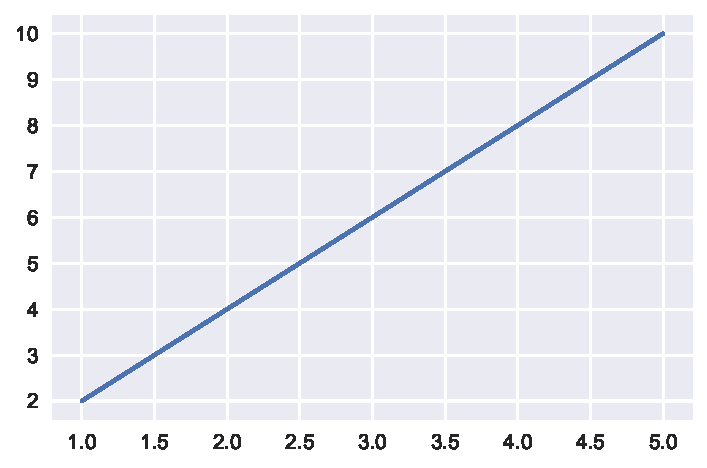
\includegraphics{index_files/figure-pdf/cell-2-output-1.pdf}

}

\end{figure}

\hypertarget{gruxe1ficos-de-barras}{%
\subsection{Gráficos de barras}\label{gruxe1ficos-de-barras}}

Los gráficos de barras son una excelente forma de representar datos
categóricos y comparar diferentes valores entre categorías. Son ideales
cuando queremos mostrar la relación entre una variable independiente
(categoría) y una variable dependiente (valor).

\textbf{Paso 1: Preparar los datos} Antes de crear el gráfico de barras,
necesitamos tener nuestros datos organizados. Asegúrate de tener una
lista o array con las categorías que deseas representar en el eje X, y
otra lista o array con los valores correspondientes en el eje Y.

\textbf{Paso 2: Crear el gráfico} Utilizaremos la función \texttt{bar()}
de Matplotlib para crear el gráfico de barras. Pasaremos nuestros datos
de los ejes X e Y como argumentos. A continuación, utilizaremos la
función \texttt{show()} para visualizar el gráfico.

\begin{Shaded}
\begin{Highlighting}[]
\ImportTok{import}\NormalTok{ matplotlib.pyplot }\ImportTok{as}\NormalTok{ plt}

\CommentTok{\# Datos de ejemplo}
\NormalTok{categorias }\OperatorTok{=}\NormalTok{ [}\StringTok{\textquotesingle{}A\textquotesingle{}}\NormalTok{, }\StringTok{\textquotesingle{}B\textquotesingle{}}\NormalTok{, }\StringTok{\textquotesingle{}C\textquotesingle{}}\NormalTok{, }\StringTok{\textquotesingle{}D\textquotesingle{}}\NormalTok{]}
\NormalTok{valores }\OperatorTok{=}\NormalTok{ [}\DecValTok{10}\NormalTok{, }\DecValTok{15}\NormalTok{, }\DecValTok{7}\NormalTok{, }\DecValTok{12}\NormalTok{]}

\CommentTok{\# Crear el gráfico de barras}
\NormalTok{plt.bar(categorias, valores)}

\CommentTok{\# Mostrar el gráfico}
\NormalTok{plt.show()}
\end{Highlighting}
\end{Shaded}

\begin{figure}[H]

{\centering 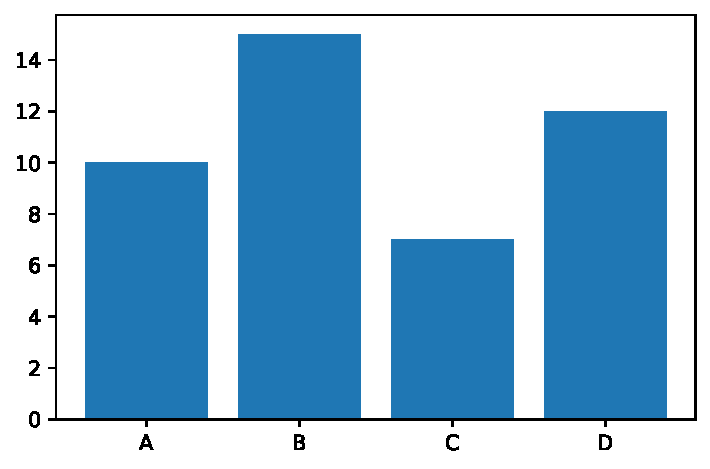
\includegraphics{index_files/figure-pdf/cell-3-output-1.pdf}

}

\end{figure}

\hypertarget{gruxe1ficos-de-dispersiuxf3n}{%
\subsection{Gráficos de dispersión}\label{gruxe1ficos-de-dispersiuxf3n}}

Los gráficos de dispersión son una excelente opción cuando queremos
visualizar la relación entre dos variables numéricas. Son especialmente
útiles para identificar patrones, tendencias o la existencia de alguna
correlación entre los datos.

\textbf{Paso 1: Preparar los datos} Antes de crear el gráfico de
dispersión, debemos asegurarnos de tener dos conjuntos de datos: uno
para el eje X (variable independiente) y otro para el eje Y (variable
dependiente). Asegúrate de que ambos conjuntos tengan la misma longitud
y correspondencia adecuada.

\textbf{Paso 2: Crear el gráfico} Utilizaremos la función
\texttt{scatter()} de Matplotlib para crear el gráfico de dispersión.
Pasaremos nuestros datos de los ejes X e Y como argumentos. Luego,
utilizaremos la función \texttt{show()} para visualizar el gráfico.

\begin{Shaded}
\begin{Highlighting}[]
\ImportTok{import}\NormalTok{ matplotlib.pyplot }\ImportTok{as}\NormalTok{ plt}

\CommentTok{\# Datos de ejemplo}
\NormalTok{x }\OperatorTok{=}\NormalTok{ [}\DecValTok{1}\NormalTok{, }\DecValTok{2}\NormalTok{, }\DecValTok{3}\NormalTok{, }\DecValTok{4}\NormalTok{, }\DecValTok{5}\NormalTok{]}
\NormalTok{y }\OperatorTok{=}\NormalTok{ [}\DecValTok{4}\NormalTok{, }\DecValTok{7}\NormalTok{, }\DecValTok{2}\NormalTok{, }\DecValTok{9}\NormalTok{, }\DecValTok{5}\NormalTok{]}

\CommentTok{\# Crear el gráfico de dispersión}
\NormalTok{plt.scatter(x, y)}

\CommentTok{\# Mostrar el gráfico}
\NormalTok{plt.show()}
\end{Highlighting}
\end{Shaded}

\begin{figure}[H]

{\centering 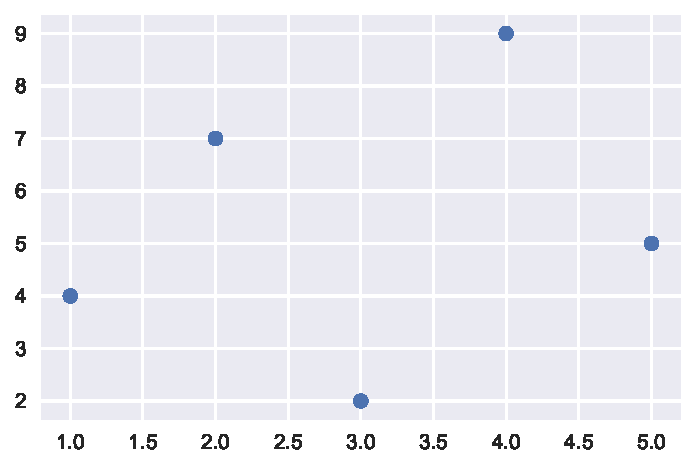
\includegraphics{index_files/figure-pdf/cell-4-output-1.pdf}

}

\end{figure}

\hypertarget{gruxe1ficos-de-uxe1rea}{%
\subsection{Gráficos de área}\label{gruxe1ficos-de-uxe1rea}}

Los gráficos de área son una forma efectiva de visualizar la
distribución o acumulación de datos a lo largo de una variable. Estos
gráficos son útiles cuando queremos mostrar la contribución relativa de
diferentes categorías o variables a un total.

\textbf{Paso 1: Preparar los datos} Antes de crear el gráfico de área,
debemos tener un conjunto de datos que represente las diferentes
categorías o variables que queremos visualizar. También necesitaremos
los valores correspondientes para cada categoría o variable.

\textbf{Paso 2: Crear el gráfico} Utilizaremos la función
\texttt{fill\_between()} de Matplotlib para crear el gráfico de área.
Pasaremos los datos de los ejes X e Y como argumentos y especificaremos
el color del área. Luego, utilizaremos la función \texttt{show()} para
visualizar el gráfico.

\begin{Shaded}
\begin{Highlighting}[]
\ImportTok{import}\NormalTok{ matplotlib.pyplot }\ImportTok{as}\NormalTok{ plt}

\CommentTok{\# Datos de ejemplo}
\NormalTok{x }\OperatorTok{=}\NormalTok{ [}\DecValTok{1}\NormalTok{, }\DecValTok{2}\NormalTok{, }\DecValTok{3}\NormalTok{, }\DecValTok{4}\NormalTok{, }\DecValTok{5}\NormalTok{]}
\NormalTok{y }\OperatorTok{=}\NormalTok{ [}\DecValTok{2}\NormalTok{, }\DecValTok{4}\NormalTok{, }\DecValTok{6}\NormalTok{, }\DecValTok{4}\NormalTok{, }\DecValTok{8}\NormalTok{]}

\CommentTok{\# Crear el gráfico de área}
\NormalTok{plt.fill\_between(x, y, color}\OperatorTok{=}\StringTok{\textquotesingle{}skyblue\textquotesingle{}}\NormalTok{)}

\CommentTok{\# Mostrar el gráfico}
\NormalTok{plt.show()}
\end{Highlighting}
\end{Shaded}

\begin{figure}[H]

{\centering 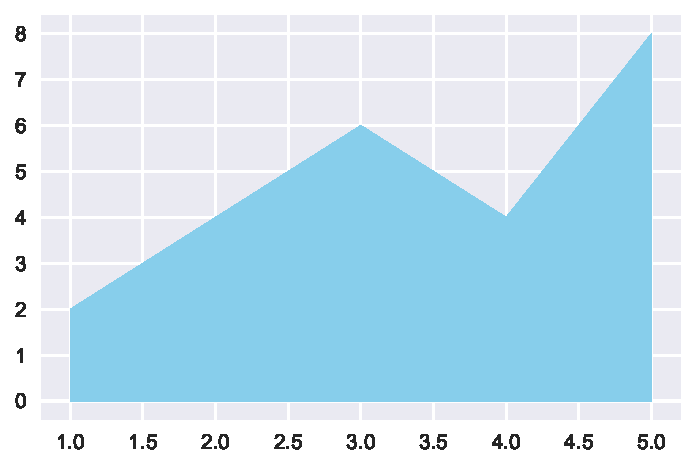
\includegraphics{index_files/figure-pdf/cell-5-output-1.pdf}

}

\end{figure}

\hypertarget{gruxe1ficos-de-pastel}{%
\subsection{Gráficos de pastel}\label{gruxe1ficos-de-pastel}}

Los gráficos de pastel son una forma popular de visualizar la proporción
de diferentes categorías o variables en un conjunto de datos. Estos
gráficos circulares son útiles para representar datos que se dividen en
partes proporcionales.

\textbf{Paso 1: Preparar los datos} Antes de crear el gráfico de pastel,
debemos tener un conjunto de datos con las categorías o variables que
queremos representar y los valores correspondientes para cada una de
ellas.

\textbf{Paso 2: Crear el gráfico} Utilizaremos la función \texttt{pie()}
de Matplotlib para crear el gráfico de pastel. Pasaremos los valores de
las categorías como argumentos y especificaremos los colores y etiquetas
correspondientes. Luego, utilizaremos la función \texttt{show()} para
visualizar el gráfico.

\begin{Shaded}
\begin{Highlighting}[]
\ImportTok{import}\NormalTok{ matplotlib.pyplot }\ImportTok{as}\NormalTok{ plt}

\CommentTok{\# Datos de ejemplo}
\NormalTok{categorias }\OperatorTok{=}\NormalTok{ [}\StringTok{\textquotesingle{}Manzanas\textquotesingle{}}\NormalTok{, }\StringTok{\textquotesingle{}Naranjas\textquotesingle{}}\NormalTok{, }\StringTok{\textquotesingle{}Plátanos\textquotesingle{}}\NormalTok{]}
\NormalTok{valores }\OperatorTok{=}\NormalTok{ [}\DecValTok{30}\NormalTok{, }\DecValTok{40}\NormalTok{, }\DecValTok{20}\NormalTok{]}

\CommentTok{\# Crear el gráfico de pastel}
\NormalTok{plt.pie(valores, labels}\OperatorTok{=}\NormalTok{categorias, colors}\OperatorTok{=}\NormalTok{[}\StringTok{\textquotesingle{}red\textquotesingle{}}\NormalTok{, }\StringTok{\textquotesingle{}orange\textquotesingle{}}\NormalTok{, }\StringTok{\textquotesingle{}yellow\textquotesingle{}}\NormalTok{])}

\CommentTok{\# Mostrar el gráfico}
\NormalTok{plt.show()}
\end{Highlighting}
\end{Shaded}

\begin{figure}[H]

{\centering 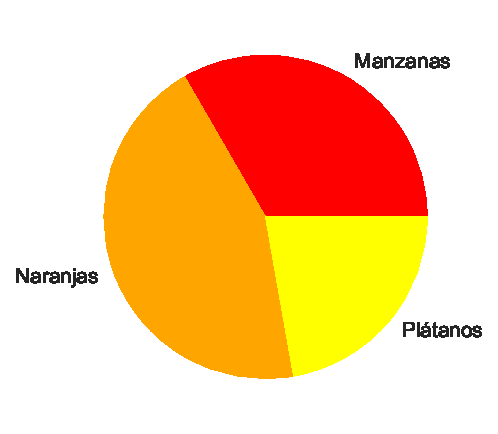
\includegraphics{index_files/figure-pdf/cell-6-output-1.pdf}

}

\end{figure}

\hypertarget{personalizaciuxf3n-de-gruxe1ficos}{%
\section{Personalización de
gráficos}\label{personalizaciuxf3n-de-gruxe1ficos}}

\hypertarget{cambio-de-colores-y-estilos}{%
\subsection{Cambio de colores y
estilos}\label{cambio-de-colores-y-estilos}}

La personalización de colores y estilos en los gráficos es una forma de
agregar tu toque personal y hacer que tus visualizaciones sean más
atractivas y significativas. Con Python, puedes cambiar fácilmente los
colores de las líneas, los puntos y las áreas en tus gráficos, así como
también aplicar diferentes estilos para resaltar la información más
relevante.

\textbf{Cambio de colores:}

Puedes cambiar los colores predeterminados de tus gráficos utilizando la
opción \texttt{color} en las funciones de trazado. Por ejemplo, si
deseas cambiar el color de una línea en un gráfico de línea, puedes
especificar un color diferente utilizando el argumento \texttt{color}
seguido del nombre del color o su código hexadecimal.

\begin{Shaded}
\begin{Highlighting}[]
\ImportTok{import}\NormalTok{ matplotlib.pyplot }\ImportTok{as}\NormalTok{ plt}

\CommentTok{\# Datos de ejemplo}
\NormalTok{x }\OperatorTok{=}\NormalTok{ [}\DecValTok{1}\NormalTok{, }\DecValTok{2}\NormalTok{, }\DecValTok{3}\NormalTok{, }\DecValTok{4}\NormalTok{]}
\NormalTok{y }\OperatorTok{=}\NormalTok{ [}\DecValTok{10}\NormalTok{, }\DecValTok{20}\NormalTok{, }\DecValTok{15}\NormalTok{, }\DecValTok{25}\NormalTok{]}

\CommentTok{\# Cambiar el color de la línea a rojo}
\NormalTok{plt.plot(x, y, color}\OperatorTok{=}\StringTok{\textquotesingle{}red\textquotesingle{}}\NormalTok{)}

\CommentTok{\# Mostrar el gráfico}
\NormalTok{plt.show()}
\end{Highlighting}
\end{Shaded}

\begin{figure}[H]

{\centering 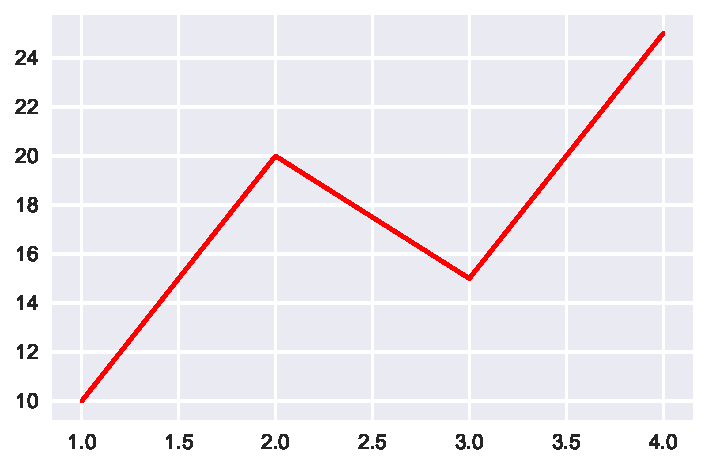
\includegraphics{index_files/figure-pdf/cell-7-output-1.pdf}

}

\end{figure}

Además de los colores predefinidos, también puedes utilizar códigos
hexadecimales para seleccionar colores personalizados. Por ejemplo,
\texttt{color=\textquotesingle{}\#FF0000\textquotesingle{}} representa
el color rojo.

\textbf{Cambio de estilos:}

Python también te permite cambiar el estilo de tus gráficos para
adaptarlos a tus preferencias. Puedes utilizar diferentes estilos
predefinidos, como \texttt{\textquotesingle{}seaborn\textquotesingle{}},
\texttt{\textquotesingle{}ggplot\textquotesingle{}},
\texttt{\textquotesingle{}fivethirtyeight\textquotesingle{}}, entre
otros. Simplemente utiliza la función \texttt{plt.style.use()} y pasa el
nombre del estilo que deseas aplicar.

\begin{Shaded}
\begin{Highlighting}[]
\ImportTok{import}\NormalTok{ matplotlib.pyplot }\ImportTok{as}\NormalTok{ plt}

\CommentTok{\# Estilo de gráfico \textquotesingle{}seaborn\textquotesingle{}}
\NormalTok{plt.style.use(}\StringTok{\textquotesingle{}seaborn\textquotesingle{}}\NormalTok{)}

\CommentTok{\# Datos y trazado del gráfico}
\NormalTok{x }\OperatorTok{=}\NormalTok{ [}\DecValTok{1}\NormalTok{, }\DecValTok{2}\NormalTok{, }\DecValTok{3}\NormalTok{, }\DecValTok{4}\NormalTok{]}
\NormalTok{y }\OperatorTok{=}\NormalTok{ [}\DecValTok{10}\NormalTok{, }\DecValTok{20}\NormalTok{, }\DecValTok{15}\NormalTok{, }\DecValTok{25}\NormalTok{]}
\NormalTok{plt.plot(x, y)}

\CommentTok{\# Mostrar el gráfico}
\NormalTok{plt.show()}
\end{Highlighting}
\end{Shaded}

\begin{figure}[H]

{\centering 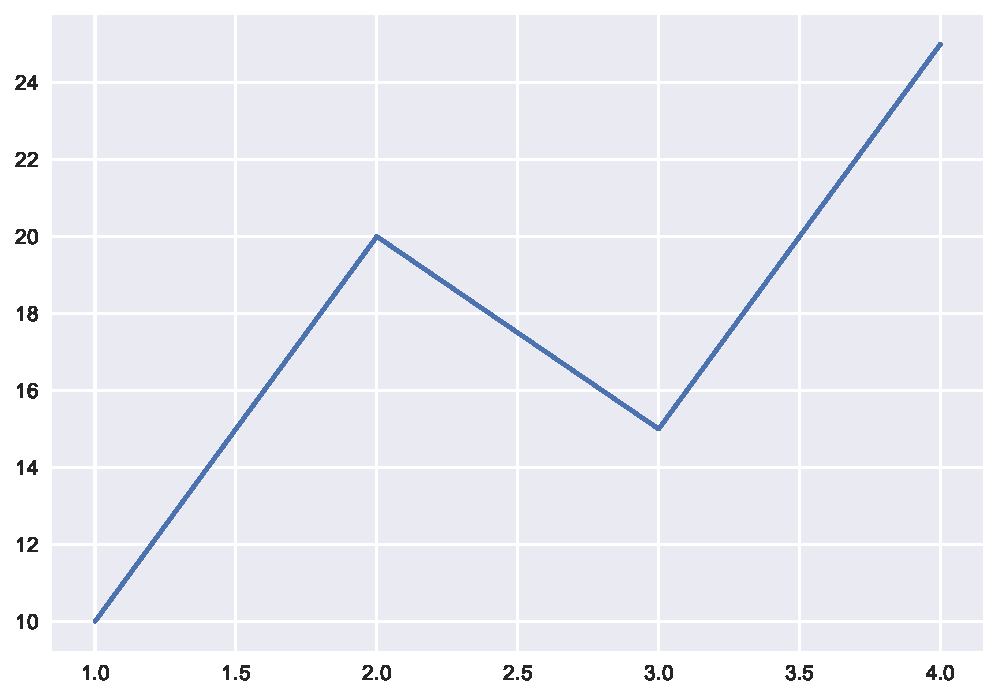
\includegraphics{index_files/figure-pdf/cell-8-output-1.pdf}

}

\end{figure}

Puedes experimentar con diferentes estilos y encontrar el que se ajuste
mejor a tus necesidades y preferencias.

\hypertarget{agregando-etiquetas-y-tuxedtulos}{%
\subsection{Agregando etiquetas y
títulos}\label{agregando-etiquetas-y-tuxedtulos}}

Las etiquetas y los títulos son elementos clave en tus gráficos, ya que
proporcionan información adicional y ayudan a interpretar los datos de
manera más clara. Python te ofrece varias opciones para agregar
etiquetas a los ejes, así como títulos para el gráfico en general.

\textbf{Etiquetas de ejes:}

Las etiquetas de ejes son fundamentales para comprender qué representan
los valores en los gráficos. Puedes agregar etiquetas a los ejes x e y
utilizando las funciones \texttt{plt.xlabel()} y \texttt{plt.ylabel()},
respectivamente. Simplemente pasa una cadena de texto como argumento
para describir cada eje.

\begin{Shaded}
\begin{Highlighting}[]
\ImportTok{import}\NormalTok{ matplotlib.pyplot }\ImportTok{as}\NormalTok{ plt}

\CommentTok{\# Datos de ejemplo}
\NormalTok{x }\OperatorTok{=}\NormalTok{ [}\DecValTok{1}\NormalTok{, }\DecValTok{2}\NormalTok{, }\DecValTok{3}\NormalTok{, }\DecValTok{4}\NormalTok{]}
\NormalTok{y }\OperatorTok{=}\NormalTok{ [}\DecValTok{10}\NormalTok{, }\DecValTok{20}\NormalTok{, }\DecValTok{15}\NormalTok{, }\DecValTok{25}\NormalTok{]}

\CommentTok{\# Trazado del gráfico}
\NormalTok{plt.plot(x, y)}

\CommentTok{\# Etiquetas de ejes}
\NormalTok{plt.xlabel(}\StringTok{\textquotesingle{}Eje X\textquotesingle{}}\NormalTok{)}
\NormalTok{plt.ylabel(}\StringTok{\textquotesingle{}Eje Y\textquotesingle{}}\NormalTok{)}

\CommentTok{\# Mostrar el gráfico}
\NormalTok{plt.show()}
\end{Highlighting}
\end{Shaded}

\begin{figure}[H]

{\centering 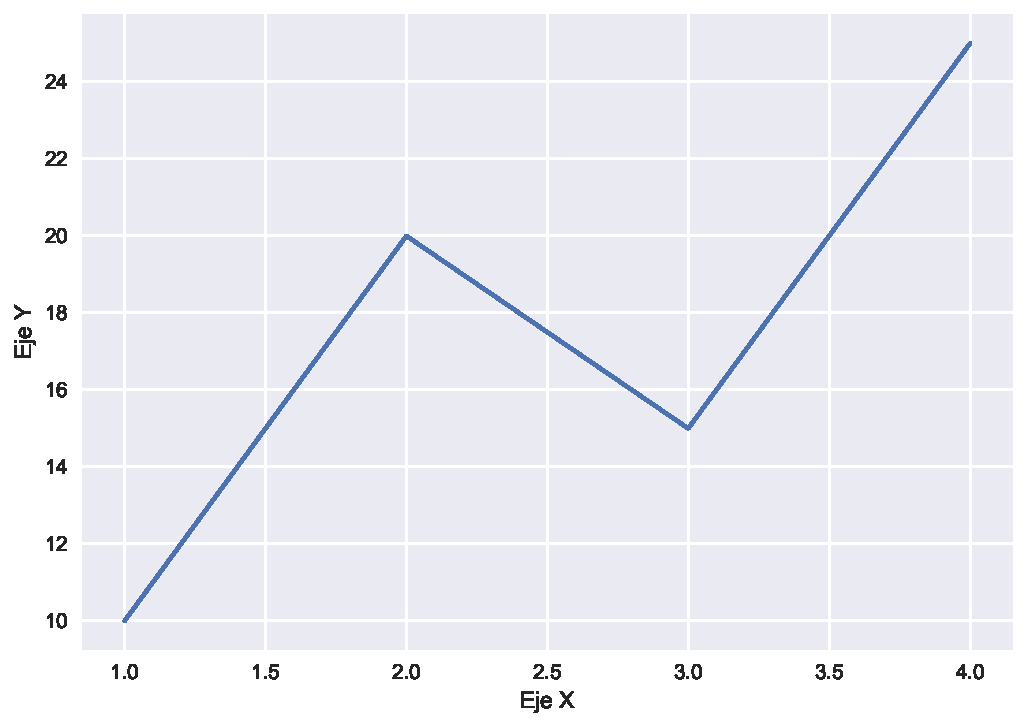
\includegraphics{index_files/figure-pdf/cell-9-output-1.pdf}

}

\end{figure}

Asegúrate de elegir etiquetas descriptivas que reflejen el contenido y
la interpretación de los datos en tus gráficos.

\textbf{Título del gráfico:}

El título del gráfico es útil para resumir la información principal o el
propósito del gráfico. Puedes agregar un título utilizando la función
\texttt{plt.title()} y pasando una cadena de texto como argumento.

\begin{Shaded}
\begin{Highlighting}[]
\ImportTok{import}\NormalTok{ matplotlib.pyplot }\ImportTok{as}\NormalTok{ plt}

\CommentTok{\# Datos de ejemplo}
\NormalTok{x }\OperatorTok{=}\NormalTok{ [}\DecValTok{1}\NormalTok{, }\DecValTok{2}\NormalTok{, }\DecValTok{3}\NormalTok{, }\DecValTok{4}\NormalTok{]}
\NormalTok{y }\OperatorTok{=}\NormalTok{ [}\DecValTok{10}\NormalTok{, }\DecValTok{20}\NormalTok{, }\DecValTok{15}\NormalTok{, }\DecValTok{25}\NormalTok{]}

\CommentTok{\# Trazado del gráfico}
\NormalTok{plt.plot(x, y)}

\CommentTok{\# Título del gráfico}
\NormalTok{plt.title(}\StringTok{\textquotesingle{}Gráfico de ejemplo\textquotesingle{}}\NormalTok{)}

\CommentTok{\# Mostrar el gráfico}
\NormalTok{plt.show()}
\end{Highlighting}
\end{Shaded}

\begin{figure}[H]

{\centering 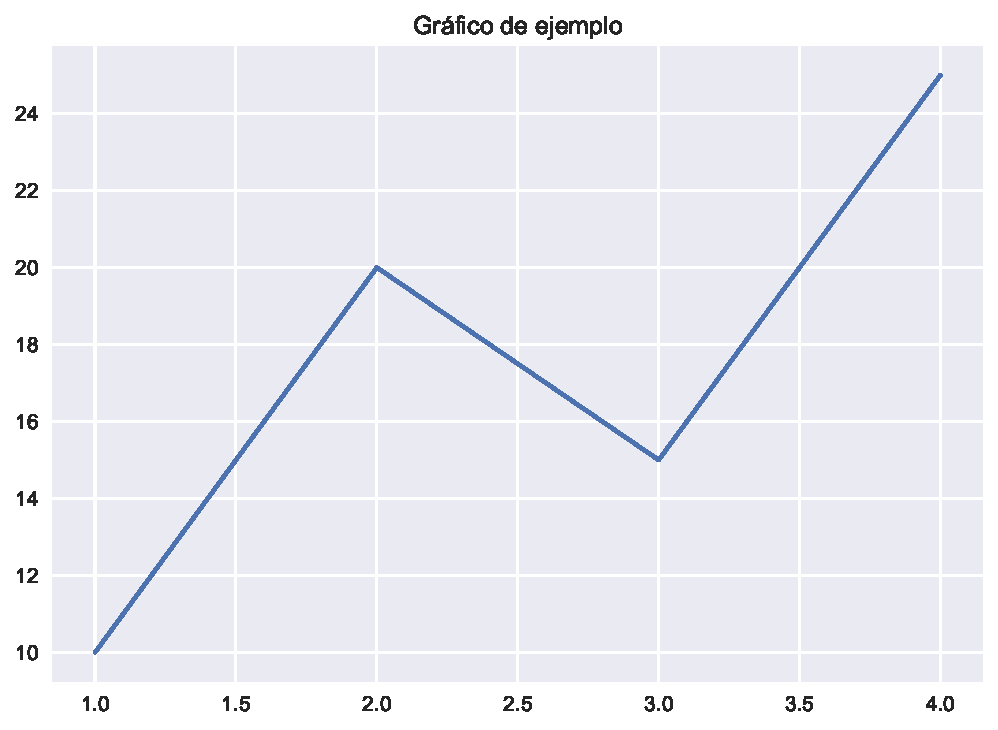
\includegraphics{index_files/figure-pdf/cell-10-output-1.pdf}

}

\end{figure}

Al igual que con las etiquetas de ejes, elige un título claro y conciso
que resuma la información que se muestra en el gráfico.

\hypertarget{configuraciuxf3n-de-ejes-y-leyendas}{%
\subsection{Configuración de ejes y
leyendas}\label{configuraciuxf3n-de-ejes-y-leyendas}}

La configuración de los ejes y las leyendas en tus gráficos es
fundamental para proporcionar más información y claridad a tus
visualizaciones. Python te ofrece diversas opciones para personalizar
los ejes y agregar leyendas que ayuden a interpretar tus gráficos de
manera efectiva.

\textbf{Personalización de ejes:}

Puedes personalizar los ejes de tu gráfico mediante la función
\texttt{plt.axis()}, que te permite establecer los límites de los ejes x
e y. Pasa una lista en el siguiente orden:
\texttt{{[}xmin,\ xmax,\ ymin,\ ymax{]}} para definir los límites de
cada eje.

\begin{Shaded}
\begin{Highlighting}[]
\ImportTok{import}\NormalTok{ matplotlib.pyplot }\ImportTok{as}\NormalTok{ plt}

\CommentTok{\# Datos de ejemplo}
\NormalTok{x }\OperatorTok{=}\NormalTok{ [}\DecValTok{1}\NormalTok{, }\DecValTok{2}\NormalTok{, }\DecValTok{3}\NormalTok{, }\DecValTok{4}\NormalTok{]}
\NormalTok{y }\OperatorTok{=}\NormalTok{ [}\DecValTok{10}\NormalTok{, }\DecValTok{20}\NormalTok{, }\DecValTok{15}\NormalTok{, }\DecValTok{25}\NormalTok{]}

\CommentTok{\# Trazado del gráfico}
\NormalTok{plt.plot(x, y)}

\CommentTok{\# Personalización de ejes}
\NormalTok{plt.axis([}\DecValTok{0}\NormalTok{, }\DecValTok{5}\NormalTok{, }\DecValTok{0}\NormalTok{, }\DecValTok{30}\NormalTok{])}

\CommentTok{\# Mostrar el gráfico}
\NormalTok{plt.show()}
\end{Highlighting}
\end{Shaded}

\begin{figure}[H]

{\centering 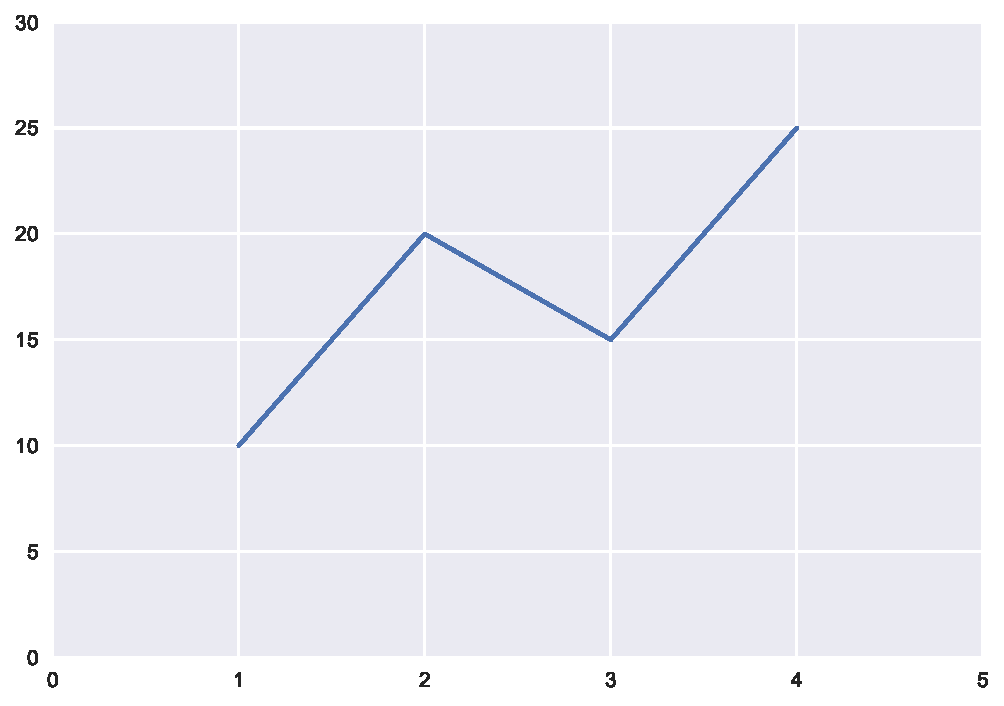
\includegraphics{index_files/figure-pdf/cell-11-output-1.pdf}

}

\end{figure}

Establecer límites adecuados en los ejes es importante para asegurarte
de que tus datos se muestren correctamente y se ajusten al espacio
disponible en el gráfico.

\textbf{Agregando leyendas:}

Las leyendas son útiles para identificar diferentes elementos en tus
gráficos, como líneas, barras o puntos. Puedes agregar una leyenda
utilizando la función \texttt{plt.legend()} después de trazar los
elementos en tu gráfico. Además, puedes especificar la ubicación de la
leyenda pasando un argumento como
\texttt{\textquotesingle{}upper\ right\textquotesingle{}},
\texttt{\textquotesingle{}lower\ left\textquotesingle{}}, etc.

\begin{Shaded}
\begin{Highlighting}[]
\ImportTok{import}\NormalTok{ matplotlib.pyplot }\ImportTok{as}\NormalTok{ plt}

\CommentTok{\# Datos de ejemplo}
\NormalTok{x }\OperatorTok{=}\NormalTok{ [}\DecValTok{1}\NormalTok{, }\DecValTok{2}\NormalTok{, }\DecValTok{3}\NormalTok{, }\DecValTok{4}\NormalTok{]}
\NormalTok{y1 }\OperatorTok{=}\NormalTok{ [}\DecValTok{10}\NormalTok{, }\DecValTok{20}\NormalTok{, }\DecValTok{15}\NormalTok{, }\DecValTok{25}\NormalTok{]}
\NormalTok{y2 }\OperatorTok{=}\NormalTok{ [}\DecValTok{5}\NormalTok{, }\DecValTok{15}\NormalTok{, }\DecValTok{10}\NormalTok{, }\DecValTok{20}\NormalTok{]}

\CommentTok{\# Trazado del gráfico}
\NormalTok{plt.plot(x, y1, label}\OperatorTok{=}\StringTok{\textquotesingle{}Serie 1\textquotesingle{}}\NormalTok{)}
\NormalTok{plt.plot(x, y2, label}\OperatorTok{=}\StringTok{\textquotesingle{}Serie 2\textquotesingle{}}\NormalTok{)}

\CommentTok{\# Agregar leyenda}
\NormalTok{plt.legend(loc}\OperatorTok{=}\StringTok{\textquotesingle{}upper right\textquotesingle{}}\NormalTok{)}

\CommentTok{\# Mostrar el gráfico}
\NormalTok{plt.show()}
\end{Highlighting}
\end{Shaded}

\begin{figure}[H]

{\centering 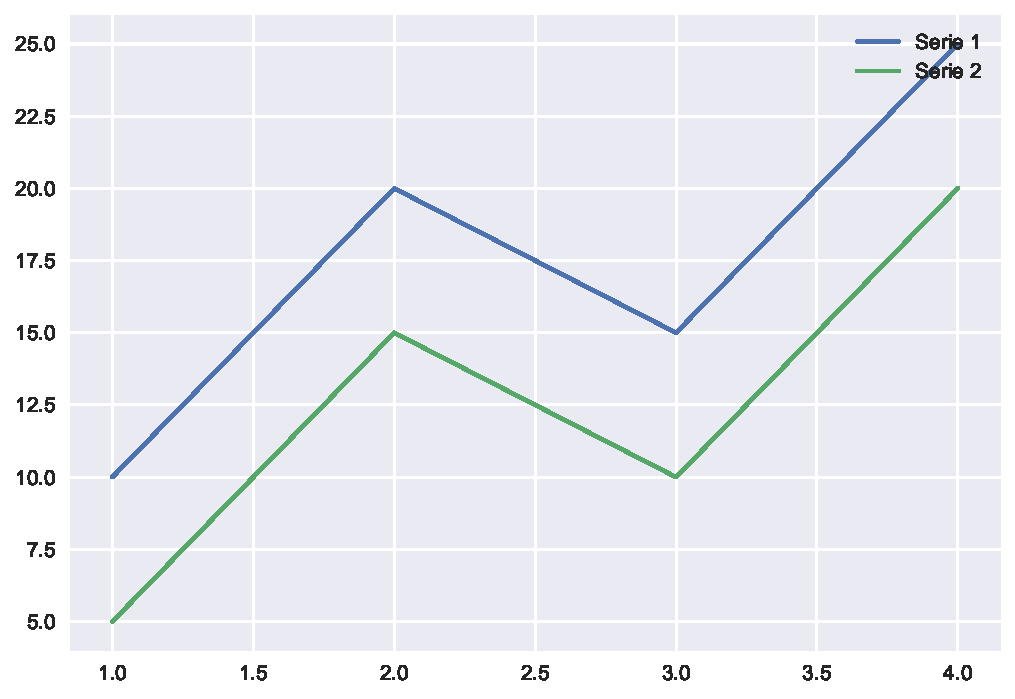
\includegraphics{index_files/figure-pdf/cell-12-output-1.pdf}

}

\end{figure}

Asegúrate de proporcionar etiquetas claras para cada serie de datos en
tu gráfico. Esto ayudará a los lectores a comprender qué representa cada
línea o elemento visualizado.

\hypertarget{auxf1adiendo-anotaciones-y-texto}{%
\subsection{Añadiendo anotaciones y
texto}\label{auxf1adiendo-anotaciones-y-texto}}

Las anotaciones y el texto son una forma poderosa de resaltar puntos
clave o proporcionar información adicional en tus gráficos. Python te
ofrece diversas opciones para añadir anotaciones y texto de manera
sencilla y efectiva.

\textbf{Anotaciones:}

Puedes añadir anotaciones en puntos específicos de tu gráfico utilizando
la función \texttt{plt.annotate()}. Esta función te permite colocar
texto en coordenadas específicas del gráfico. Puedes especificar las
coordenadas \texttt{xy} del punto donde deseas colocar la anotación y
las coordenadas \texttt{xytext} donde deseas que aparezca el texto.

\begin{Shaded}
\begin{Highlighting}[]
\ImportTok{import}\NormalTok{ matplotlib.pyplot }\ImportTok{as}\NormalTok{ plt}

\CommentTok{\# Datos de ejemplo}
\NormalTok{x }\OperatorTok{=}\NormalTok{ [}\DecValTok{1}\NormalTok{, }\DecValTok{2}\NormalTok{, }\DecValTok{3}\NormalTok{, }\DecValTok{4}\NormalTok{]}
\NormalTok{y }\OperatorTok{=}\NormalTok{ [}\DecValTok{10}\NormalTok{, }\DecValTok{20}\NormalTok{, }\DecValTok{15}\NormalTok{, }\DecValTok{25}\NormalTok{]}

\CommentTok{\# Trazado del gráfico}
\NormalTok{plt.plot(x, y)}

\CommentTok{\# Añadir una anotación}
\NormalTok{plt.annotate(}\StringTok{\textquotesingle{}Punto importante\textquotesingle{}}\NormalTok{, xy}\OperatorTok{=}\NormalTok{(}\DecValTok{2}\NormalTok{, }\DecValTok{20}\NormalTok{), xytext}\OperatorTok{=}\NormalTok{(}\DecValTok{3}\NormalTok{, }\DecValTok{22}\NormalTok{),}
\NormalTok{             arrowprops}\OperatorTok{=}\BuiltInTok{dict}\NormalTok{(arrowstyle}\OperatorTok{=}\StringTok{\textquotesingle{}{-}\textgreater{}\textquotesingle{}}\NormalTok{))}

\CommentTok{\# Mostrar el gráfico}
\NormalTok{plt.show()}
\end{Highlighting}
\end{Shaded}

\begin{figure}[H]

{\centering 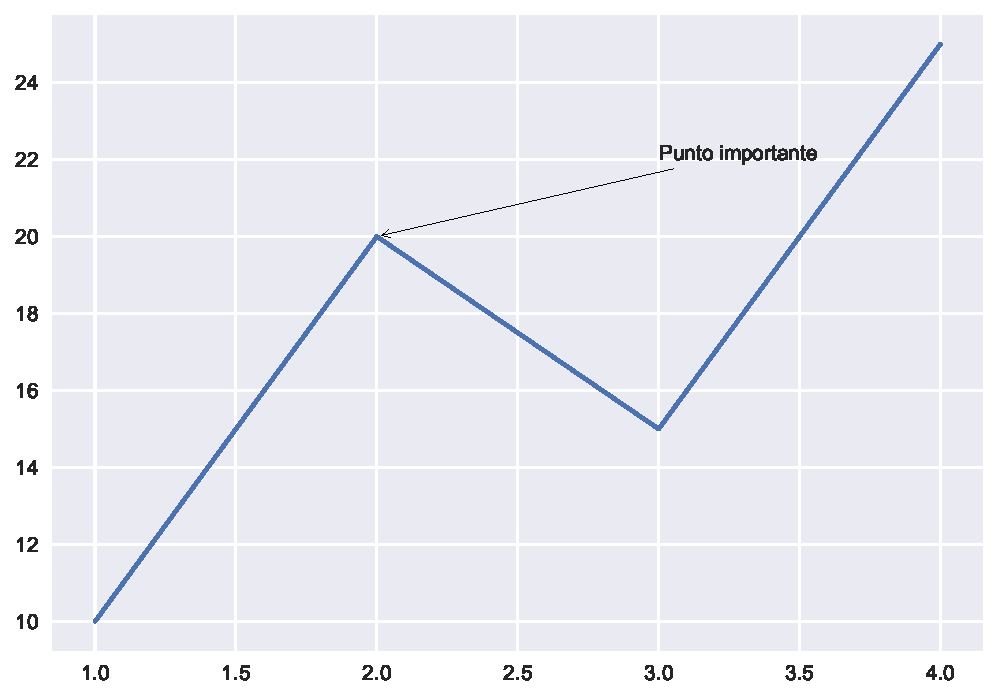
\includegraphics{index_files/figure-pdf/cell-13-output-1.pdf}

}

\end{figure}

Puedes personalizar aún más las anotaciones agregando flechas utilizando
el parámetro \texttt{arrowprops}. Esto puede ayudar a resaltar la
relación entre la anotación y el punto correspondiente en el gráfico.

\textbf{Texto:}

Además de las anotaciones, también puedes agregar texto en ubicaciones
específicas utilizando la función \texttt{plt.text()}. Esta función te
permite colocar texto en cualquier posición del gráfico especificando
las coordenadas \texttt{x} e \texttt{y} del punto donde deseas que
aparezca el texto.

\begin{Shaded}
\begin{Highlighting}[]
\ImportTok{import}\NormalTok{ matplotlib.pyplot }\ImportTok{as}\NormalTok{ plt}

\CommentTok{\# Datos de ejemplo}
\NormalTok{x }\OperatorTok{=}\NormalTok{ [}\DecValTok{1}\NormalTok{, }\DecValTok{2}\NormalTok{, }\DecValTok{3}\NormalTok{, }\DecValTok{4}\NormalTok{]}
\NormalTok{y }\OperatorTok{=}\NormalTok{ [}\DecValTok{10}\NormalTok{, }\DecValTok{20}\NormalTok{, }\DecValTok{15}\NormalTok{, }\DecValTok{25}\NormalTok{]}

\CommentTok{\# Trazado del gráfico}
\NormalTok{plt.plot(x, y)}

\CommentTok{\# Añadir texto}
\NormalTok{plt.text(}\DecValTok{2}\NormalTok{, }\DecValTok{20}\NormalTok{, }\StringTok{\textquotesingle{}Texto adicional\textquotesingle{}}\NormalTok{, fontsize}\OperatorTok{=}\DecValTok{12}\NormalTok{)}

\CommentTok{\# Mostrar el gráfico}
\NormalTok{plt.show()}
\end{Highlighting}
\end{Shaded}

\begin{figure}[H]

{\centering 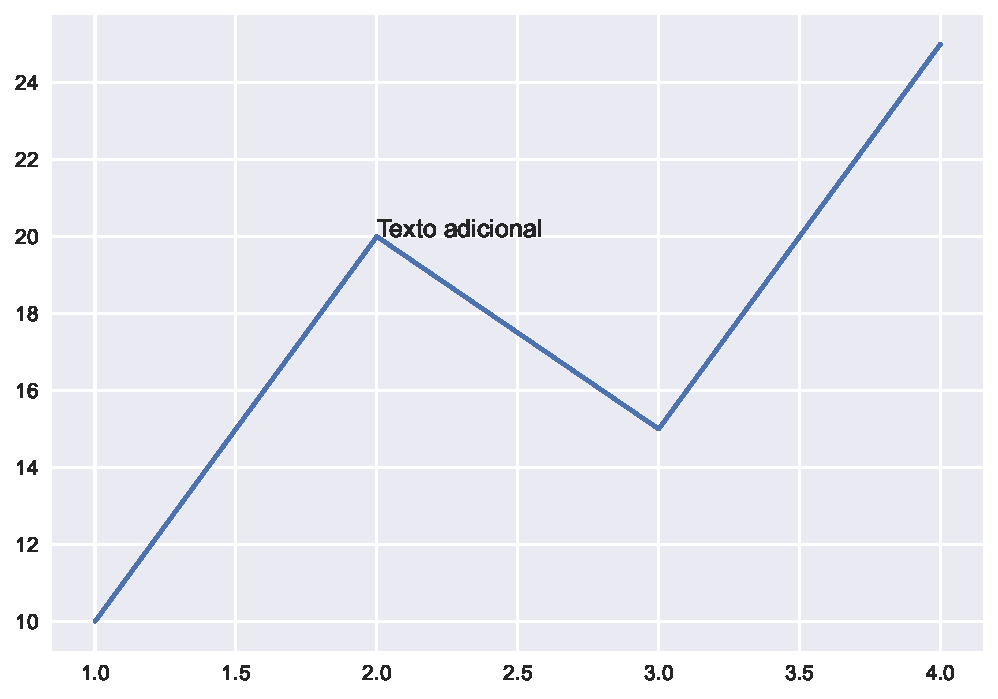
\includegraphics{index_files/figure-pdf/cell-14-output-1.pdf}

}

\end{figure}

Puedes ajustar el tamaño de la fuente del texto mediante el parámetro
\texttt{fontsize} para asegurarte de que sea legible y se ajuste a tu
gráfico.

\hypertarget{gruxe1ficos-avanzados}{%
\section{Gráficos avanzados}\label{gruxe1ficos-avanzados}}

\hypertarget{gruxe1ficos-de-contorno}{%
\subsection{Gráficos de contorno}\label{gruxe1ficos-de-contorno}}

Los gráficos de contorno son una forma efectiva de visualizar datos
tridimensionales en un formato bidimensional. Estos gráficos utilizan
líneas de contorno para representar las diferentes regiones de valores
en un plano.

En Python, puedes crear gráficos de contorno utilizando la función
\texttt{plt.contour()} de Matplotlib. Esta función toma los datos en
forma de matrices 2D y genera el gráfico de contorno correspondiente.

\begin{Shaded}
\begin{Highlighting}[]
\ImportTok{import}\NormalTok{ matplotlib.pyplot }\ImportTok{as}\NormalTok{ plt}
\ImportTok{import}\NormalTok{ numpy }\ImportTok{as}\NormalTok{ np}

\CommentTok{\# Datos de ejemplo}
\NormalTok{x }\OperatorTok{=}\NormalTok{ np.linspace(}\OperatorTok{{-}}\DecValTok{2}\NormalTok{, }\DecValTok{2}\NormalTok{, }\DecValTok{100}\NormalTok{)}
\NormalTok{y }\OperatorTok{=}\NormalTok{ np.linspace(}\OperatorTok{{-}}\DecValTok{2}\NormalTok{, }\DecValTok{2}\NormalTok{, }\DecValTok{100}\NormalTok{)}
\NormalTok{X, Y }\OperatorTok{=}\NormalTok{ np.meshgrid(x, y)}
\NormalTok{Z }\OperatorTok{=}\NormalTok{ np.sin(X}\OperatorTok{**}\DecValTok{2} \OperatorTok{+}\NormalTok{ Y}\OperatorTok{**}\DecValTok{2}\NormalTok{)}

\CommentTok{\# Crear gráfico de contorno}
\NormalTok{plt.contour(X, Y, Z)}

\CommentTok{\# Personalizar el gráfico}
\NormalTok{plt.title(}\StringTok{\textquotesingle{}Gráfico de contorno\textquotesingle{}}\NormalTok{)}
\NormalTok{plt.xlabel(}\StringTok{\textquotesingle{}Eje X\textquotesingle{}}\NormalTok{)}
\NormalTok{plt.ylabel(}\StringTok{\textquotesingle{}Eje Y\textquotesingle{}}\NormalTok{)}

\CommentTok{\# Mostrar el gráfico}
\NormalTok{plt.show()}
\end{Highlighting}
\end{Shaded}

\begin{figure}[H]

{\centering 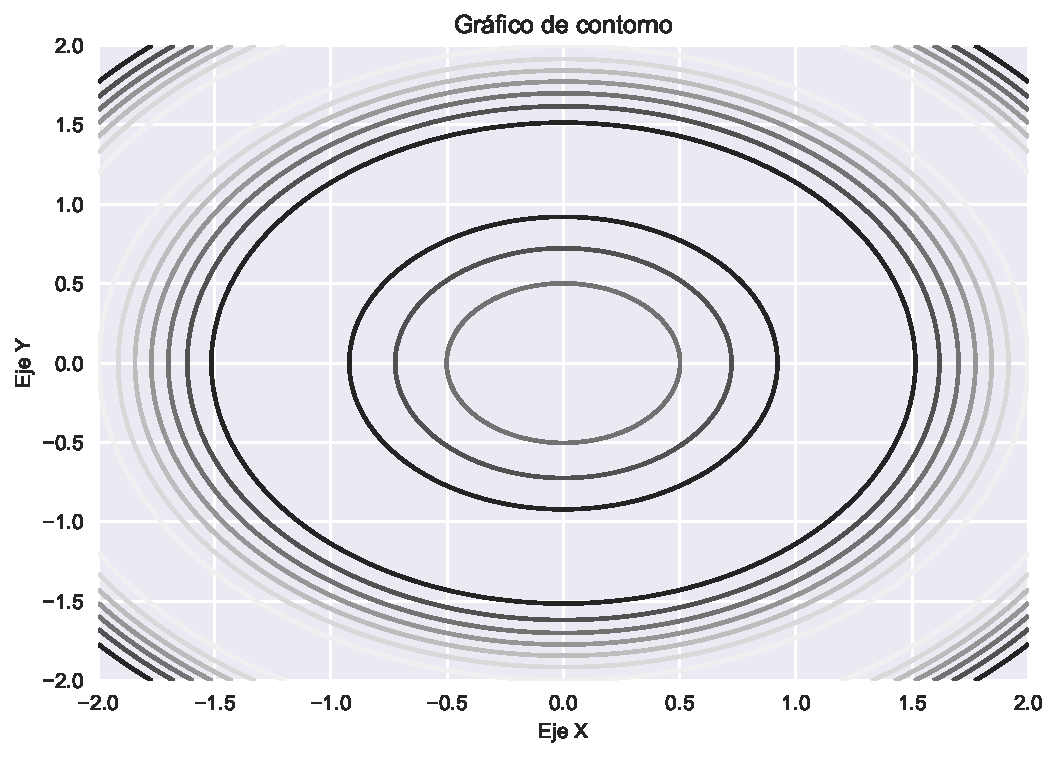
\includegraphics{index_files/figure-pdf/cell-15-output-1.pdf}

}

\end{figure}

En el código anterior, creamos una matriz 2D de valores \texttt{Z}
basados en los valores de las matrices \texttt{X} e \texttt{Y}. Luego
utilizamos \texttt{plt.contour()} para trazar el gráfico de contorno.
Puedes ajustar la apariencia del gráfico personalizando los títulos de
los ejes y agregando etiquetas.

Los gráficos de contorno son útiles para visualizar relaciones y
patrones en datos tridimensionales de manera más comprensible. Puedes
experimentar con diferentes configuraciones y colores para resaltar
áreas específicas o ajustar los niveles de contorno para obtener más
detalles.

\hypertarget{gruxe1ficos-3d}{%
\subsection{Gráficos 3D}\label{gruxe1ficos-3d}}

Los gráficos 3D son una forma visualmente impactante de representar
datos en tres dimensiones. Estos gráficos nos permiten explorar
relaciones complejas y patrones en nuestros datos de una manera más
inmersiva.

En Python, podemos crear gráficos 3D utilizando la biblioteca
Matplotlib. La función \texttt{plt.plot\_surface()} nos permite trazar
superficies 3D a partir de matrices de datos.

\begin{Shaded}
\begin{Highlighting}[]
\ImportTok{import}\NormalTok{ matplotlib.pyplot }\ImportTok{as}\NormalTok{ plt}
\ImportTok{import}\NormalTok{ numpy }\ImportTok{as}\NormalTok{ np}

\CommentTok{\# Datos de ejemplo}
\NormalTok{x }\OperatorTok{=}\NormalTok{ np.linspace(}\OperatorTok{{-}}\DecValTok{5}\NormalTok{, }\DecValTok{5}\NormalTok{, }\DecValTok{100}\NormalTok{)}
\NormalTok{y }\OperatorTok{=}\NormalTok{ np.linspace(}\OperatorTok{{-}}\DecValTok{5}\NormalTok{, }\DecValTok{5}\NormalTok{, }\DecValTok{100}\NormalTok{)}
\NormalTok{X, Y }\OperatorTok{=}\NormalTok{ np.meshgrid(x, y)}
\NormalTok{Z }\OperatorTok{=}\NormalTok{ np.sin(np.sqrt(X}\OperatorTok{**}\DecValTok{2} \OperatorTok{+}\NormalTok{ Y}\OperatorTok{**}\DecValTok{2}\NormalTok{))}

\CommentTok{\# Crear gráfico 3D}
\NormalTok{fig }\OperatorTok{=}\NormalTok{ plt.figure()}
\NormalTok{ax }\OperatorTok{=}\NormalTok{ fig.add\_subplot(}\DecValTok{111}\NormalTok{, projection}\OperatorTok{=}\StringTok{\textquotesingle{}3d\textquotesingle{}}\NormalTok{)}
\NormalTok{ax.plot\_surface(X, Y, Z)}

\CommentTok{\# Personalizar el gráfico}
\NormalTok{ax.set\_title(}\StringTok{\textquotesingle{}Gráfico 3D\textquotesingle{}}\NormalTok{)}
\NormalTok{ax.set\_xlabel(}\StringTok{\textquotesingle{}Eje X\textquotesingle{}}\NormalTok{)}
\NormalTok{ax.set\_ylabel(}\StringTok{\textquotesingle{}Eje Y\textquotesingle{}}\NormalTok{)}
\NormalTok{ax.set\_zlabel(}\StringTok{\textquotesingle{}Eje Z\textquotesingle{}}\NormalTok{)}

\CommentTok{\# Mostrar el gráfico}
\NormalTok{plt.show()}
\end{Highlighting}
\end{Shaded}

\begin{figure}[H]

{\centering 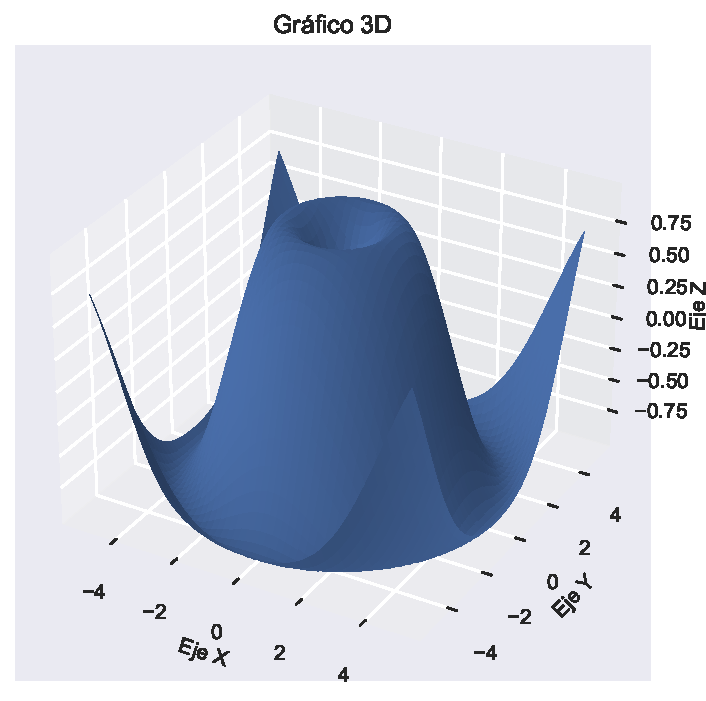
\includegraphics{index_files/figure-pdf/cell-16-output-1.pdf}

}

\end{figure}

En el código anterior, creamos matrices \texttt{X}, \texttt{Y} y
\texttt{Z} que representan los puntos de la superficie tridimensional.
Luego, utilizamos \texttt{plt.plot\_surface()} junto con la proyección
\texttt{\textquotesingle{}3d\textquotesingle{}} para trazar la
superficie en el gráfico 3D.

Puedes personalizar el gráfico ajustando los títulos de los ejes y
agregando etiquetas según sea necesario. Además, puedes experimentar con
diferentes configuraciones, como cambiar los colores, ajustar la
iluminación o agregar puntos de datos adicionales.

Los gráficos 3D son especialmente útiles cuando trabajamos con datos que
involucran múltiples variables. Nos permiten visualizar relaciones
complejas y descubrir patrones que podrían no ser evidentes en gráficos
bidimensionales.

\hypertarget{gruxe1ficos-de-mapas}{%
\subsection{Gráficos de mapas}\label{gruxe1ficos-de-mapas}}

Los gráficos de mapas son una forma poderosa de visualizar datos
geoespaciales y resaltar patrones y distribuciones en un mapa
interactivo. Con Python, podemos utilizar diversas bibliotecas, como
Folium o Plotly, para crear gráficos de mapas personalizados.

Una de las bibliotecas más populares para gráficos de mapas es Folium.
Esta biblioteca nos permite crear mapas interactivos utilizando datos
geoespaciales y agregar capas adicionales, como marcadores o polígonos.

\begin{Shaded}
\begin{Highlighting}[]
\CommentTok{\# pip install folium}
\ImportTok{import}\NormalTok{ folium}

\CommentTok{\# Crear un mapa}
\NormalTok{mapa }\OperatorTok{=}\NormalTok{ folium.Map(location}\OperatorTok{=}\NormalTok{[}\FloatTok{40.7128}\NormalTok{, }\OperatorTok{{-}}\FloatTok{74.0060}\NormalTok{], zoom\_start}\OperatorTok{=}\DecValTok{10}\NormalTok{)}

\CommentTok{\# Agregar un marcador}
\NormalTok{folium.Marker(location}\OperatorTok{=}\NormalTok{[}\FloatTok{40.7128}\NormalTok{, }\OperatorTok{{-}}\FloatTok{74.0060}\NormalTok{], popup}\OperatorTok{=}\StringTok{\textquotesingle{}Nueva York\textquotesingle{}}\NormalTok{).add\_to(mapa)}

\CommentTok{\# Mostrar el mapa}
\NormalTok{mapa}
\end{Highlighting}
\end{Shaded}

\begin{verbatim}
<folium.folium.Map at 0x7fac008c7ee0>
\end{verbatim}

En el código anterior, creamos un mapa centrado en una ubicación
específica (latitud y longitud) utilizando \texttt{folium.Map()}. Luego,
agregamos un marcador en la misma ubicación utilizando
\texttt{folium.Marker()}. Puedes personalizar el marcador y agregar
información adicional, como un mensaje emergente, para proporcionar más
detalles.

Folium también nos permite agregar capas adicionales, como polígonos o
rutas, utilizando funciones como \texttt{folium.Polygon()} o
\texttt{folium.PolyLine()}. Estas capas pueden ayudarnos a representar
datos geoespaciales más complejos y enriquecer nuestra visualización.

Otra biblioteca popular para gráficos de mapas es Plotly, que nos ofrece
capacidades de visualización interactiva y personalizable. Con Plotly,
podemos crear mapas con múltiples capas y utilizar técnicas de
visualización avanzadas, como el mapa de calor o la agregación espacial.

Los gráficos de mapas son especialmente útiles para visualizar datos
geoespaciales, como ubicaciones de tiendas, distribución de población o
rutas. Nos permiten comprender mejor la información cuando está
relacionada con la ubicación geográfica.

\hypertarget{gruxe1ficos-interactivos}{%
\subsection{Gráficos interactivos}\label{gruxe1ficos-interactivos}}

Los gráficos interactivos son una forma fascinante de visualizar datos y
permitir a los usuarios explorar la información de manera dinámica.
Python nos ofrece varias bibliotecas poderosas para crear gráficos
interactivos, como Plotly, Bokeh y Altair.

Una de las bibliotecas más populares para gráficos interactivos es
Plotly. Esta biblioteca nos permite crear gráficos interactivos con
características como zoom, pan y herramientas para resaltar puntos de
datos específicos. Además, Plotly proporciona una interfaz sencilla para
personalizar y diseñar nuestros gráficos.

\begin{Shaded}
\begin{Highlighting}[]
\ImportTok{import}\NormalTok{ pandas }\ImportTok{as}\NormalTok{ pd}

\CommentTok{\# Definir los datos y exportamos a un .csv}
\NormalTok{datos }\OperatorTok{=}\NormalTok{ \{}
    \StringTok{\textquotesingle{}nombre\textquotesingle{}}\NormalTok{: [}\StringTok{\textquotesingle{}Juan\textquotesingle{}}\NormalTok{, }\StringTok{\textquotesingle{}María\textquotesingle{}}\NormalTok{, }\StringTok{\textquotesingle{}Carlos\textquotesingle{}}\NormalTok{, }\StringTok{\textquotesingle{}Laura\textquotesingle{}}\NormalTok{],}
    \StringTok{\textquotesingle{}edad\textquotesingle{}}\NormalTok{: [}\DecValTok{25}\NormalTok{, }\DecValTok{30}\NormalTok{, }\DecValTok{35}\NormalTok{, }\DecValTok{28}\NormalTok{],}
    \StringTok{\textquotesingle{}salario\textquotesingle{}}\NormalTok{: [}\DecValTok{50000}\NormalTok{, }\DecValTok{60000}\NormalTok{, }\DecValTok{70000}\NormalTok{, }\DecValTok{55000}\NormalTok{],}
    \StringTok{\textquotesingle{}departamento\textquotesingle{}}\NormalTok{: [}\StringTok{\textquotesingle{}Ventas\textquotesingle{}}\NormalTok{, }\StringTok{\textquotesingle{}Marketing\textquotesingle{}}\NormalTok{, }\StringTok{\textquotesingle{}Finanzas\textquotesingle{}}\NormalTok{, }\StringTok{\textquotesingle{}Recursos Humanos\textquotesingle{}}\NormalTok{]}
\NormalTok{\}}

\CommentTok{\# Crear un DataFrame con los datos}
\NormalTok{df }\OperatorTok{=}\NormalTok{ pd.DataFrame(datos)}

\CommentTok{\# Guardar el DataFrame en un archivo CSV}
\NormalTok{df.to\_csv(}\StringTok{\textquotesingle{}datos.csv\textquotesingle{}}\NormalTok{, index}\OperatorTok{=}\VariableTok{False}\NormalTok{)}
\end{Highlighting}
\end{Shaded}

\begin{Shaded}
\begin{Highlighting}[]
\ImportTok{import}\NormalTok{ pandas }\ImportTok{as}\NormalTok{ pd}
\ImportTok{import}\NormalTok{ plotly.express }\ImportTok{as}\NormalTok{ px}

\NormalTok{df }\OperatorTok{=}\NormalTok{ pd.read\_csv(}\StringTok{\textquotesingle{}datos.csv\textquotesingle{}}\NormalTok{)}

\CommentTok{\# Crear un gráfico interactivo de dispersión}
\NormalTok{fig }\OperatorTok{=}\NormalTok{ px.scatter(df, x}\OperatorTok{=}\StringTok{"edad"}\NormalTok{, y}\OperatorTok{=}\StringTok{"salario"}\NormalTok{, color}\OperatorTok{=}\StringTok{"departamento"}\NormalTok{, hover\_data}\OperatorTok{=}\NormalTok{[}\StringTok{"nombre"}\NormalTok{])}

\CommentTok{\# Personalizar el diseño y las herramientas interactivas}
\NormalTok{fig.update\_layout(}
\NormalTok{    title}\OperatorTok{=}\StringTok{"Relación entre edad, salario y departamento"}\NormalTok{,}
\NormalTok{    xaxis\_title}\OperatorTok{=}\StringTok{"Edad"}\NormalTok{,}
\NormalTok{    yaxis\_title}\OperatorTok{=}\StringTok{"Salario"}\NormalTok{,}
\NormalTok{    hovermode}\OperatorTok{=}\StringTok{"closest"}
\NormalTok{)}

\CommentTok{\# Mostrar el gráfico interactivo}
\NormalTok{fig.show()}
\end{Highlighting}
\end{Shaded}

\begin{verbatim}
Unable to display output for mime type(s): text/html
\end{verbatim}

\begin{verbatim}
Unable to display output for mime type(s): text/html
\end{verbatim}

En el código anterior, utilizamos la biblioteca Plotly Express para
crear un gráfico interactivo de dispersión. Especificamos las columnas
del DataFrame que deseamos visualizar y personalizamos el gráfico con
títulos, etiquetas y configuraciones de interacción.

Además de Plotly, Bokeh y Altair también son bibliotecas populares para
crear gráficos interactivos en Python. Bokeh nos permite crear
visualizaciones interactivas basadas en navegadores web, mientras que
Altair se centra en la creación de gráficos declarativos y basados en
gramáticas.

Los gráficos interactivos son ideales para explorar datos, ya que
permiten a los usuarios interactuar con los gráficos y profundizar en la
información. Pueden ser utilizados para resaltar puntos de datos,
mostrar detalles adicionales en herramientas emergentes o incluso para
filtrar y seleccionar subconjuntos de datos.

\hypertarget{visualizaciuxf3n-de-datos-en-tiempo-real}{%
\section{Visualización de datos en tiempo
real}\label{visualizaciuxf3n-de-datos-en-tiempo-real}}

\hypertarget{uso-de-bibliotecas-para-datos-en-continuo}{%
\subsection{Uso de bibliotecas para datos en
continuo}\label{uso-de-bibliotecas-para-datos-en-continuo}}

La visualización de datos en tiempo real es una técnica poderosa para
analizar y monitorear datos que evolucionan constantemente. Python
ofrece varias bibliotecas que nos permiten visualizar datos en continuo
y actualizar gráficos en tiempo real.

Una de las bibliotecas más utilizadas para visualización en tiempo real
es Matplotlib. Aunque Matplotlib es conocida principalmente por crear
gráficos estáticos, también podemos aprovechar sus capacidades para
visualizar datos en tiempo real. Podemos utilizar la función
\texttt{plt.plot()} en un bucle mientras los datos se actualizan
continuamente para lograr la visualización en tiempo real.

\begin{Shaded}
\begin{Highlighting}[]
\ImportTok{import}\NormalTok{ matplotlib.pyplot }\ImportTok{as}\NormalTok{ plt}
\ImportTok{import}\NormalTok{ numpy }\ImportTok{as}\NormalTok{ np}

\CommentTok{\# Configuración inicial}
\NormalTok{fig, ax }\OperatorTok{=}\NormalTok{ plt.subplots()}
\NormalTok{x }\OperatorTok{=}\NormalTok{ np.linspace(}\DecValTok{0}\NormalTok{, }\DecValTok{10}\NormalTok{, }\DecValTok{100}\NormalTok{)}
\NormalTok{y }\OperatorTok{=}\NormalTok{ np.sin(x)}

\CommentTok{\# Actualización en tiempo real}
\ControlFlowTok{for}\NormalTok{ i }\KeywordTok{in} \BuiltInTok{range}\NormalTok{(}\DecValTok{100}\NormalTok{):}
\NormalTok{    y }\OperatorTok{=}\NormalTok{ np.sin(x }\OperatorTok{+}\NormalTok{ i }\OperatorTok{*} \FloatTok{0.1}\NormalTok{)}
\NormalTok{    ax.clear()}
\NormalTok{    ax.plot(x, y)}
\NormalTok{    plt.pause(}\FloatTok{0.1}\NormalTok{)}

\NormalTok{plt.show()}
\end{Highlighting}
\end{Shaded}

\begin{figure}[H]

{\centering 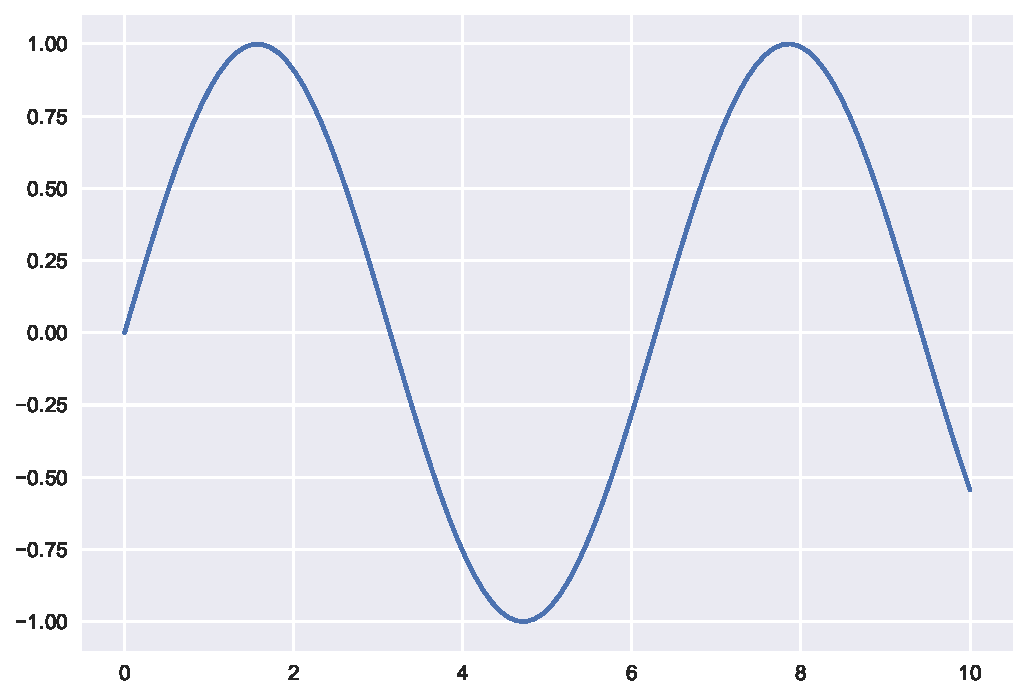
\includegraphics{index_files/figure-pdf/cell-20-output-1.pdf}

}

\end{figure}

En el código anterior, utilizamos Matplotlib para crear un gráfico de
línea en tiempo real. En cada iteración del bucle, actualizamos los
datos y redibujamos el gráfico utilizando \texttt{ax.clear()} para
eliminar el contenido anterior y \texttt{ax.plot()} para trazar los
nuevos datos. Luego, utilizamos \texttt{plt.pause()} para pausar
brevemente la ejecución y permitir la actualización visual.

Otra biblioteca popular para visualización en tiempo real es Bokeh.
Bokeh nos permite crear gráficos interactivos y actualizables en un
navegador web. Con su funcionalidad de streaming de datos, podemos
conectar nuestros datos en continuo y observar cómo evolucionan en
tiempo real.

\begin{Shaded}
\begin{Highlighting}[]
\ImportTok{from}\NormalTok{ bokeh.plotting }\ImportTok{import}\NormalTok{ figure, curdoc}
\ImportTok{from}\NormalTok{ bokeh.models }\ImportTok{import}\NormalTok{ ColumnDataSource}
\ImportTok{import}\NormalTok{ numpy }\ImportTok{as}\NormalTok{ np}

\CommentTok{\# Configuración inicial}
\NormalTok{p }\OperatorTok{=}\NormalTok{ figure()}
\NormalTok{x }\OperatorTok{=}\NormalTok{ np.linspace(}\DecValTok{0}\NormalTok{, }\DecValTok{10}\NormalTok{, }\DecValTok{100}\NormalTok{)}
\NormalTok{y }\OperatorTok{=}\NormalTok{ np.sin(x)}

\CommentTok{\# Actualización en tiempo real}
\NormalTok{source }\OperatorTok{=}\NormalTok{ ColumnDataSource(data}\OperatorTok{=}\BuiltInTok{dict}\NormalTok{(x}\OperatorTok{=}\NormalTok{x, y}\OperatorTok{=}\NormalTok{y))}
\NormalTok{p.line(x}\OperatorTok{=}\StringTok{\textquotesingle{}x\textquotesingle{}}\NormalTok{, y}\OperatorTok{=}\StringTok{\textquotesingle{}y\textquotesingle{}}\NormalTok{, source}\OperatorTok{=}\NormalTok{source)}

\KeywordTok{def}\NormalTok{ update():}
\NormalTok{    new\_y }\OperatorTok{=}\NormalTok{ np.sin(x }\OperatorTok{+}\NormalTok{ curdoc().count }\OperatorTok{*} \FloatTok{0.1}\NormalTok{)}
\NormalTok{    source.data }\OperatorTok{=} \BuiltInTok{dict}\NormalTok{(x}\OperatorTok{=}\NormalTok{x, y}\OperatorTok{=}\NormalTok{new\_y)}
\NormalTok{    curdoc().count }\OperatorTok{+=} \DecValTok{1}

\NormalTok{curdoc().count }\OperatorTok{=} \DecValTok{0}
\NormalTok{curdoc().add\_periodic\_callback(update, }\DecValTok{100}\NormalTok{)}

\NormalTok{curdoc().title }\OperatorTok{=} \StringTok{"Visualización en tiempo real"}
\NormalTok{curdoc().add\_root(p)}
\end{Highlighting}
\end{Shaded}

En este ejemplo de Bokeh, utilizamos la función \texttt{figure()} para
crear un nuevo gráfico y \texttt{p.line()} para trazar la línea inicial.
Luego, definimos una función \texttt{update()} que actualiza los datos y
los asigna a la fuente de datos \texttt{ColumnDataSource}. Utilizamos
\texttt{curdoc().add\_periodic\_callback()} para llamar a la función
\texttt{update()} periódicamente y actualizar los datos en tiempo real.

\hypertarget{actualizaciuxf3n-de-gruxe1ficos-en-tiempo-real}{%
\subsection{Actualización de gráficos en tiempo
real}\label{actualizaciuxf3n-de-gruxe1ficos-en-tiempo-real}}

Una de las características más interesantes de la visualización de datos
en tiempo real es la capacidad de actualizar los gráficos de forma
dinámica a medida que los datos cambian. Esto nos permite observar los
cambios en tiempo real y tomar decisiones basadas en la información más
reciente.

Existen diferentes enfoques para lograr la actualización de gráficos en
tiempo real, dependiendo de la biblioteca de visualización que estemos
utilizando. Veamos algunos ejemplos con las bibliotecas Matplotlib y
Bokeh.

\hypertarget{matplotlib}{%
\subsubsection{Matplotlib}\label{matplotlib}}

En Matplotlib, podemos lograr la actualización de gráficos en tiempo
real utilizando la función \texttt{plt.pause()} dentro de un bucle.
Veamos un ejemplo:

\begin{Shaded}
\begin{Highlighting}[]
\ImportTok{import}\NormalTok{ matplotlib.pyplot }\ImportTok{as}\NormalTok{ plt}
\ImportTok{import}\NormalTok{ numpy }\ImportTok{as}\NormalTok{ np}

\CommentTok{\# Configuración inicial}
\NormalTok{fig, ax }\OperatorTok{=}\NormalTok{ plt.subplots()}
\NormalTok{x }\OperatorTok{=}\NormalTok{ np.linspace(}\DecValTok{0}\NormalTok{, }\DecValTok{10}\NormalTok{, }\DecValTok{100}\NormalTok{)}
\NormalTok{y }\OperatorTok{=}\NormalTok{ np.sin(x)}

\CommentTok{\# Actualización en tiempo real}
\ControlFlowTok{for}\NormalTok{ i }\KeywordTok{in} \BuiltInTok{range}\NormalTok{(}\DecValTok{100}\NormalTok{):}
\NormalTok{    y }\OperatorTok{=}\NormalTok{ np.sin(x }\OperatorTok{+}\NormalTok{ i }\OperatorTok{*} \FloatTok{0.1}\NormalTok{)}
\NormalTok{    ax.clear()}
\NormalTok{    ax.plot(x, y)}
\NormalTok{    plt.pause(}\FloatTok{0.1}\NormalTok{)}

\NormalTok{plt.show()}
\end{Highlighting}
\end{Shaded}

\begin{figure}[H]

{\centering 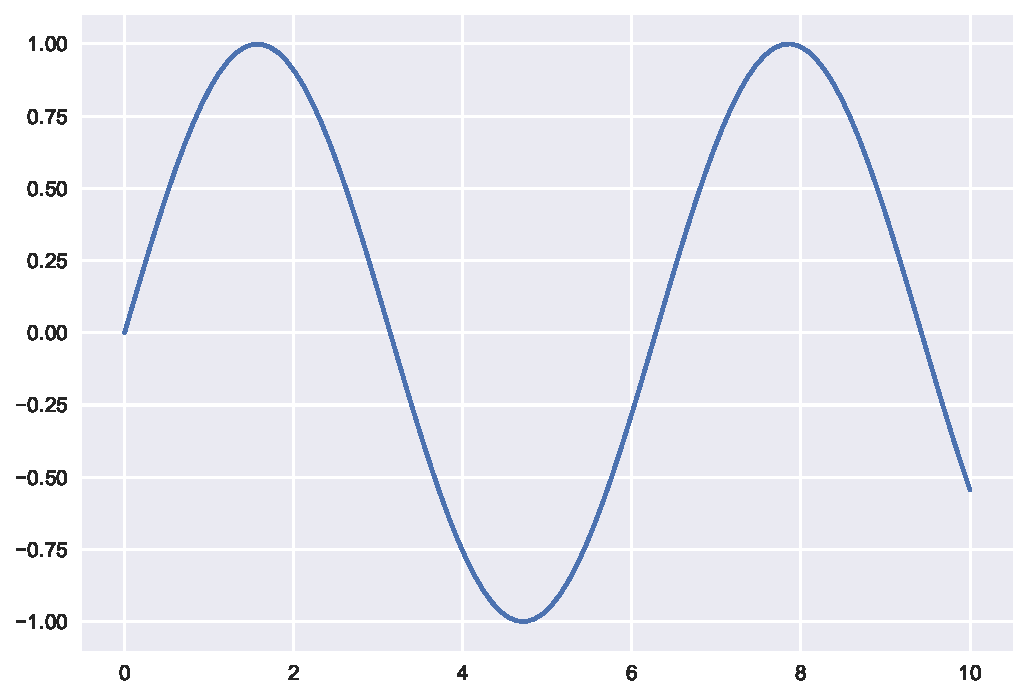
\includegraphics{index_files/figure-pdf/cell-22-output-1.pdf}

}

\end{figure}

En este ejemplo, creamos un gráfico de línea que se actualiza en tiempo
real. En cada iteración del bucle, generamos nuevos datos y los trazamos
utilizando \texttt{ax.plot()}. Utilizamos \texttt{ax.clear()} para
eliminar el contenido anterior y \texttt{plt.pause()} para pausar
brevemente la ejecución y permitir la actualización visual.

\hypertarget{bokeh}{%
\subsubsection{Bokeh}\label{bokeh}}

En Bokeh, podemos utilizar la función \texttt{ColumnDataSource} y el
método \texttt{stream()} para lograr la actualización en tiempo real.
Veamos un ejemplo:

\begin{Shaded}
\begin{Highlighting}[]
\ImportTok{from}\NormalTok{ bokeh.plotting }\ImportTok{import}\NormalTok{ figure, curdoc}
\ImportTok{from}\NormalTok{ bokeh.models }\ImportTok{import}\NormalTok{ ColumnDataSource}
\ImportTok{import}\NormalTok{ numpy }\ImportTok{as}\NormalTok{ np}

\CommentTok{\# Configuración inicial}
\NormalTok{p }\OperatorTok{=}\NormalTok{ figure()}
\NormalTok{x }\OperatorTok{=}\NormalTok{ np.linspace(}\DecValTok{0}\NormalTok{, }\DecValTok{10}\NormalTok{, }\DecValTok{100}\NormalTok{)}
\NormalTok{y }\OperatorTok{=}\NormalTok{ np.sin(x)}

\CommentTok{\# Actualización en tiempo real}
\NormalTok{source }\OperatorTok{=}\NormalTok{ ColumnDataSource(data}\OperatorTok{=}\BuiltInTok{dict}\NormalTok{(x}\OperatorTok{=}\NormalTok{x, y}\OperatorTok{=}\NormalTok{y))}
\NormalTok{p.line(x}\OperatorTok{=}\StringTok{\textquotesingle{}x\textquotesingle{}}\NormalTok{, y}\OperatorTok{=}\StringTok{\textquotesingle{}y\textquotesingle{}}\NormalTok{, source}\OperatorTok{=}\NormalTok{source)}

\KeywordTok{def}\NormalTok{ update():}
\NormalTok{    new\_y }\OperatorTok{=}\NormalTok{ np.sin(x }\OperatorTok{+}\NormalTok{ curdoc().count }\OperatorTok{*} \FloatTok{0.1}\NormalTok{)}
\NormalTok{    source.stream(}\BuiltInTok{dict}\NormalTok{(x}\OperatorTok{=}\NormalTok{x, y}\OperatorTok{=}\NormalTok{new\_y), rollover}\OperatorTok{=}\DecValTok{100}\NormalTok{)}

\NormalTok{curdoc().count }\OperatorTok{=} \DecValTok{0}
\NormalTok{curdoc().add\_periodic\_callback(update, }\DecValTok{100}\NormalTok{)}

\NormalTok{curdoc().title }\OperatorTok{=} \StringTok{"Actualización en tiempo real"}
\NormalTok{curdoc().add\_root(p)}
\end{Highlighting}
\end{Shaded}

En este ejemplo de Bokeh, utilizamos la función
\texttt{ColumnDataSource} para almacenar nuestros datos y el método
\texttt{stream()} para actualizarlos en tiempo real. La función
\texttt{update()} genera nuevos datos y los agrega a la fuente de datos
utilizando \texttt{source.stream()}. Utilizamos
\texttt{curdoc().add\_periodic\_callback()} para llamar a la función
\texttt{update()} periódicamente y actualizar los datos en tiempo real.

\hypertarget{visualizaciuxf3n-de-datos-geoespaciales}{%
\section{Visualización de datos
geoespaciales}\label{visualizaciuxf3n-de-datos-geoespaciales}}

\hypertarget{utilizaciuxf3n-de-datos-geoespaciales}{%
\subsection{Utilización de datos
geoespaciales}\label{utilizaciuxf3n-de-datos-geoespaciales}}

La visualización de datos geoespaciales nos permite representar
información en relación con su ubicación geográfica. Esto resulta
especialmente útil cuando queremos explorar patrones, tendencias y
relaciones en datos que tienen una dimensión espacial.

Para utilizar datos geoespaciales en nuestras visualizaciones,
necesitamos fuentes de datos que contengan información geográfica, como
coordenadas de latitud y longitud, códigos postales o nombres de
ciudades. Estos datos pueden provenir de diversas fuentes, como bases de
datos especializadas, servicios de mapas en línea o conjuntos de datos
abiertos.

Una de las bibliotecas más populares para trabajar con datos
geoespaciales en Python es GeoPandas. GeoPandas es una extensión de la
biblioteca Pandas que agrega capacidades espaciales, lo que nos permite
manipular y visualizar datos geoespaciales de manera sencilla.

Veamos un ejemplo básico de cómo utilizar GeoPandas para visualizar
datos geoespaciales en un mapa:

\begin{Shaded}
\begin{Highlighting}[]
\CommentTok{\#pip install geopandas}
\ImportTok{import}\NormalTok{ geopandas }\ImportTok{as}\NormalTok{ gpd}
\ImportTok{import}\NormalTok{ matplotlib.pyplot }\ImportTok{as}\NormalTok{ plt}

\CommentTok{\# Cargar datos geoespaciales}
\NormalTok{world }\OperatorTok{=}\NormalTok{ gpd.read\_file(gpd.datasets.get\_path(}\StringTok{\textquotesingle{}naturalearth\_lowres\textquotesingle{}}\NormalTok{))}

\CommentTok{\# Visualizar mapa}
\NormalTok{world.plot()}

\CommentTok{\# Mostrar el mapa}
\NormalTok{plt.show()}
\end{Highlighting}
\end{Shaded}

\begin{figure}[H]

{\centering 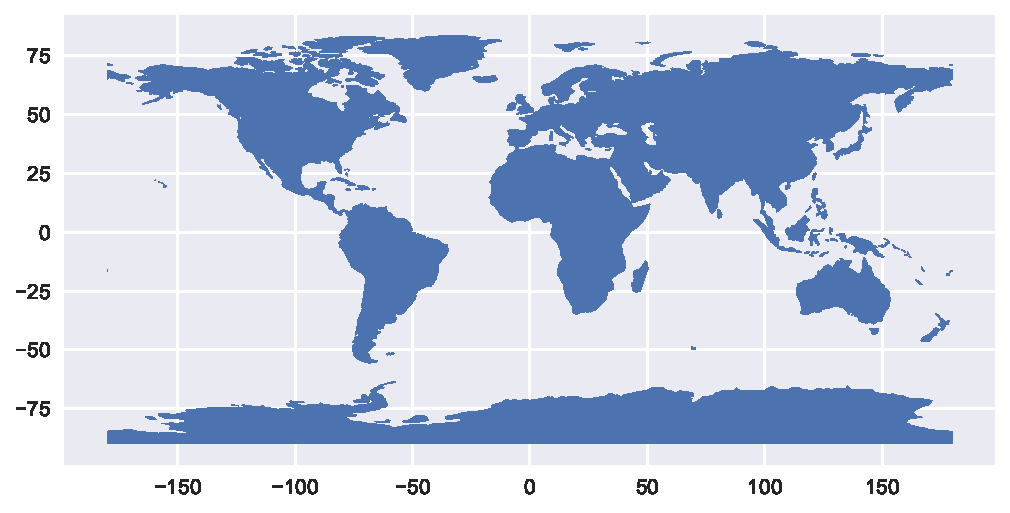
\includegraphics{index_files/figure-pdf/cell-24-output-1.pdf}

}

\end{figure}

En este ejemplo, cargamos un conjunto de datos geoespaciales que
contiene información sobre los países del mundo. Utilizamos el método
\texttt{plot()} para visualizar los datos en un mapa. Luego, utilizamos
\texttt{plt.show()} para mostrar el mapa en una ventana emergente.

Además de GeoPandas, existen otras bibliotecas como Folium y Plotly que
también nos permiten crear visualizaciones interactivas de datos
geoespaciales. Estas bibliotecas nos brindan opciones avanzadas para
personalizar los mapas, agregar capas adicionales y explorar datos de
manera interactiva.

La visualización de datos geoespaciales nos ayuda a comprender mejor la
distribución geográfica de los datos y revelar patrones ocultos que
podrían pasar desapercibidos en otro tipo de gráficos. Explorar y
visualizar datos en un contexto geoespacial agrega un nivel adicional de
información y nos permite tomar decisiones basadas en la ubicación.

\hypertarget{mapas-de-calor-y-mapas-temuxe1ticos}{%
\subsection{Mapas de calor y mapas
temáticos}\label{mapas-de-calor-y-mapas-temuxe1ticos}}

Los mapas de calor y los mapas temáticos son poderosas herramientas de
visualización que nos permiten representar datos geoespaciales de manera
más significativa. Estos mapas nos ayudan a identificar patrones y
tendencias en función de valores numéricos o categorías específicas.

Un mapa de calor utiliza colores para representar la intensidad o
densidad de un fenómeno en un área geográfica. Es ideal para mostrar la
concentración de datos o la variación espacial de una variable, como la
temperatura, la densidad de población o el rendimiento de un producto en
diferentes regiones.

Por otro lado, los mapas temáticos se utilizan para representar
categorías o clases específicas en un mapa. Cada categoría se asocia con
un color o un patrón único, lo que permite visualizar la distribución
espacial de diferentes características o atributos, como el tipo de
vegetación, la diversidad cultural o las tasas de criminalidad en
diferentes áreas.

Para crear mapas de calor y mapas temáticos, podemos utilizar
bibliotecas especializadas como Matplotlib, Seaborn y GeoPandas. Estas
bibliotecas nos brindan una variedad de funciones y herramientas para
personalizar la apariencia de nuestros mapas y resaltar la información
más relevante.

Aquí tienes un ejemplo básico de cómo crear un mapa de calor utilizando
Seaborn:

\begin{Shaded}
\begin{Highlighting}[]
\CommentTok{\#pip install seaborn matplotlib}
\ImportTok{import}\NormalTok{ seaborn }\ImportTok{as}\NormalTok{ sns}
\ImportTok{import}\NormalTok{ matplotlib.pyplot }\ImportTok{as}\NormalTok{ plt}
\ImportTok{import}\NormalTok{ numpy }\ImportTok{as}\NormalTok{ np}

\CommentTok{\# Cargar datos}
\NormalTok{data }\OperatorTok{=}\NormalTok{ np.random.rand(}\DecValTok{10}\NormalTok{, }\DecValTok{10}\NormalTok{)}

\CommentTok{\# Crear mapa de calor}
\NormalTok{sns.heatmap(data)}

\CommentTok{\# Mostrar el mapa de calor}
\NormalTok{plt.show()}
\end{Highlighting}
\end{Shaded}

\begin{figure}[H]

{\centering 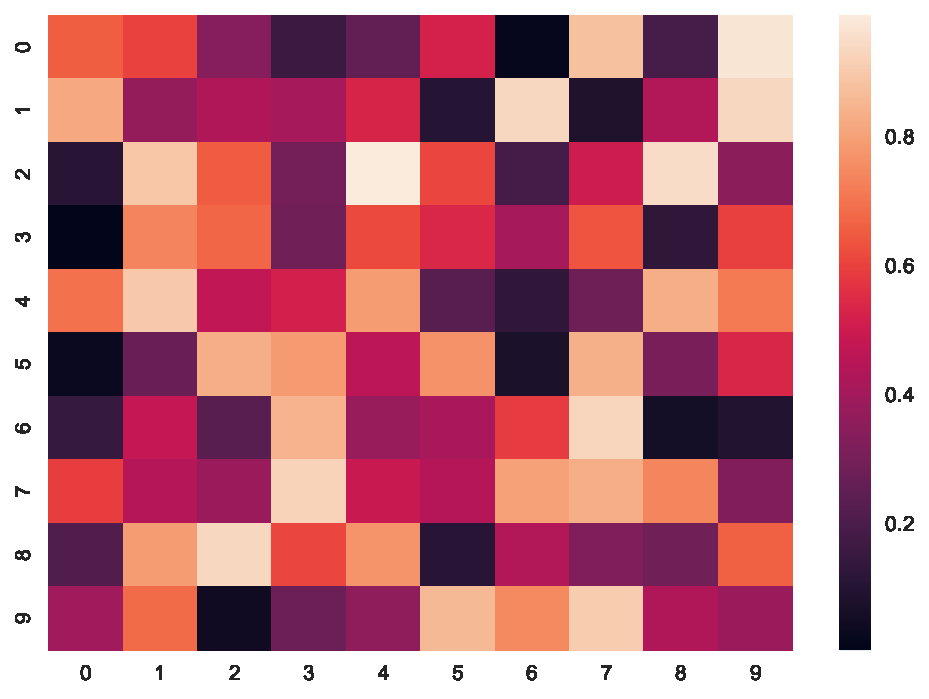
\includegraphics{index_files/figure-pdf/cell-25-output-1.pdf}

}

\end{figure}

En este ejemplo, cargamos nuestros datos y utilizamos la función
\texttt{heatmap()} de Seaborn para crear el mapa de calor. Luego,
utilizamos \texttt{plt.show()} para mostrar el mapa en una ventana
emergente.

Recuerda que la elección de colores es importante en los mapas de calor
y mapas temáticos. Debes seleccionar una paleta de colores que sea
perceptualmente equilibrada y que permita una fácil interpretación de
los datos.

Explorar datos geoespaciales a través de mapas de calor y mapas
temáticos nos brinda una visión más completa y comprensible de los
patrones y relaciones espaciales. Estas visualizaciones nos ayudan a
tomar decisiones más informadas y a comunicar eficazmente la información
a otras personas.

\hypertarget{gruxe1ficos-y-anuxe1lisis-estaduxedstico}{%
\section{Gráficos y análisis
estadístico}\label{gruxe1ficos-y-anuxe1lisis-estaduxedstico}}

\hypertarget{boxplots-y-diagramas-de-violuxedn}{%
\subsection{Boxplots y diagramas de
violín}\label{boxplots-y-diagramas-de-violuxedn}}

En el análisis de datos, a menudo necesitamos comprender la distribución
y la variabilidad de nuestros datos. Dos tipos de gráficos útiles para
visualizar esta información son los boxplots y los diagramas de violín.

Un boxplot, también conocido como diagrama de caja y bigotes, nos
proporciona una representación visual de la mediana, el rango
intercuartil (IQR) y los valores atípicos de un conjunto de datos. El
gráfico consiste en una caja que representa el IQR, una línea que
representa la mediana y dos líneas (los bigotes) que se extienden hasta
los valores mínimo y máximo dentro de un rango aceptable. Los valores
atípicos se muestran como puntos fuera de los bigotes.

Por otro lado, los diagramas de violín combinan un boxplot con una
representación de la densidad de probabilidad de los datos. Estos
gráficos muestran una forma de violín que se estrecha o ensancha según
la densidad de los datos en diferentes rangos. Esto nos proporciona
información adicional sobre la distribución y la concentración de los
datos.

Tanto los boxplots como los diagramas de violín son útiles para comparar
la distribución de diferentes grupos o categorías, identificar valores
atípicos y comprender la variabilidad en nuestros datos. Estos gráficos
nos ayudan a obtener una visión rápida y clara de la información
estadística clave.

Para crear boxplots y diagramas de violín, podemos utilizar bibliotecas
como Matplotlib y Seaborn. Estas bibliotecas nos ofrecen funciones
simples y personalizables para generar estos gráficos con facilidad.

Aquí tienes un ejemplo básico de cómo crear un boxplot utilizando
Matplotlib:

\begin{Shaded}
\begin{Highlighting}[]
\ImportTok{import}\NormalTok{ matplotlib.pyplot }\ImportTok{as}\NormalTok{ plt}
\ImportTok{import}\NormalTok{ numpy }\ImportTok{as}\NormalTok{ np}

\CommentTok{\# Cargar datos}
\NormalTok{data }\OperatorTok{=}\NormalTok{ np.random.randn(}\DecValTok{100}\NormalTok{)}

\CommentTok{\# Crear boxplot}
\NormalTok{plt.boxplot(data)}

\CommentTok{\# Mostrar el boxplot}
\NormalTok{plt.show()}
\end{Highlighting}
\end{Shaded}

\begin{figure}[H]

{\centering 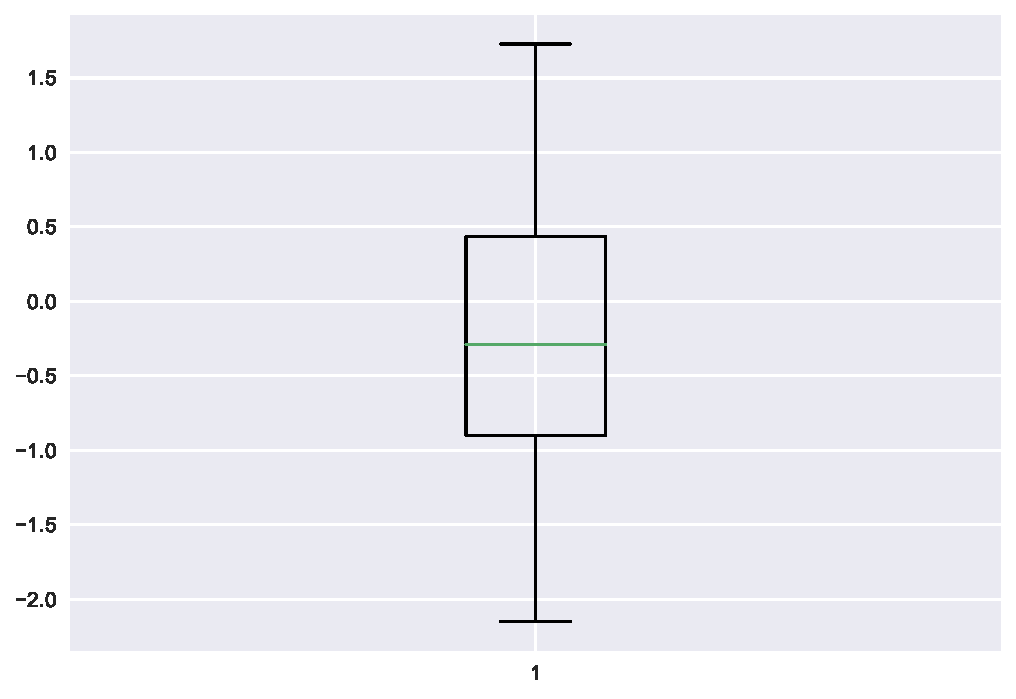
\includegraphics{index_files/figure-pdf/cell-26-output-1.pdf}

}

\end{figure}

En este ejemplo, cargamos nuestros datos y utilizamos la función
\texttt{boxplot()} de Matplotlib para crear el gráfico. Luego,
utilizamos \texttt{plt.show()} para mostrar el boxplot en una ventana
emergente.

\hypertarget{histogramas-y-distribuciones}{%
\subsection{Histogramas y
distribuciones}\label{histogramas-y-distribuciones}}

En el análisis de datos, es crucial comprender la distribución de
nuestros datos para obtener información valiosa. Una herramienta visual
poderosa para explorar la distribución es el histograma.

Un histograma es un gráfico de barras que muestra la frecuencia de
aparición de diferentes valores en un conjunto de datos. La variable que
estamos analizando se divide en intervalos y se representa en el eje x,
mientras que la frecuencia se muestra en el eje y. Cada barra representa
la cantidad de valores dentro de un intervalo específico.

Al observar un histograma, podemos identificar rápidamente la forma y la
simetría de la distribución de nuestros datos. Podemos detectar si los
datos siguen una distribución normal, están sesgados hacia la derecha o
hacia la izquierda, o si tienen múltiples picos. Esto nos proporciona
información valiosa sobre la naturaleza de nuestros datos y nos ayuda a
tomar decisiones informadas.

Para crear un histograma, podemos utilizar bibliotecas como Matplotlib y
Seaborn. Estas bibliotecas ofrecen funciones sencillas para generar
histogramas y personalizar su apariencia.

Aquí tienes un ejemplo básico de cómo crear un histograma utilizando
Matplotlib:

\begin{Shaded}
\begin{Highlighting}[]
\ImportTok{import}\NormalTok{ matplotlib.pyplot }\ImportTok{as}\NormalTok{ plt}

\CommentTok{\# Cargar datos}
\NormalTok{data }\OperatorTok{=}\NormalTok{ np.random.randn(}\DecValTok{100}\NormalTok{)}

\CommentTok{\# Crear histograma}
\NormalTok{plt.hist(data, bins}\OperatorTok{=}\DecValTok{10}\NormalTok{)  }\CommentTok{\# bins representa el número de intervalos}

\CommentTok{\# Mostrar el histograma}
\NormalTok{plt.show()}
\end{Highlighting}
\end{Shaded}

\begin{figure}[H]

{\centering 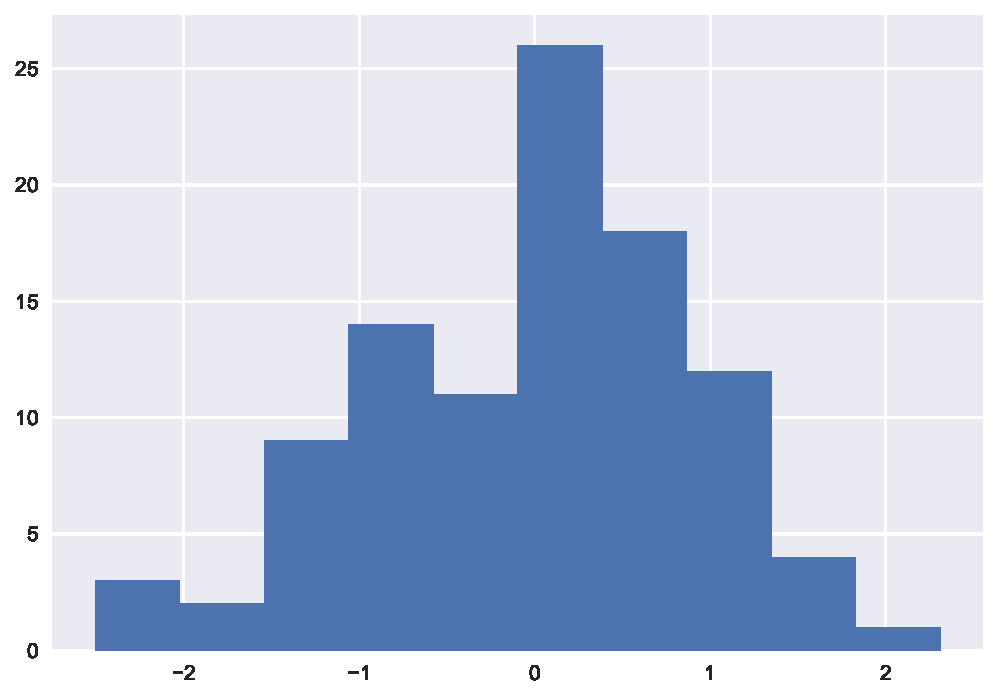
\includegraphics{index_files/figure-pdf/cell-27-output-1.pdf}

}

\end{figure}

En este ejemplo, cargamos nuestros datos y utilizamos la función
\texttt{hist()} de Matplotlib para crear el histograma. El parámetro
\texttt{bins} nos permite especificar el número de intervalos en los que
queremos dividir nuestros datos.

\hypertarget{gruxe1ficos-de-correlaciuxf3n}{%
\subsection{Gráficos de
correlación}\label{gruxe1ficos-de-correlaciuxf3n}}

Cuando trabajamos con conjuntos de datos, a menudo queremos explorar la
relación entre diferentes variables. Los gráficos de correlación nos
permiten visualizar esta relación y determinar si existe una conexión
significativa entre las variables.

Un gráfico de correlación muestra cómo se relacionan dos variables entre
sí. Nos ayuda a identificar patrones y tendencias, así como la fuerza y
dirección de la relación. El coeficiente de correlación nos proporciona
una medida numérica de la relación, donde valores cercanos a 1 indican
una correlación positiva, valores cercanos a -1 indican una correlación
negativa, y valores cercanos a 0 indican una correlación débil o
inexistente.

Una forma común de representar gráficamente la correlación es mediante
un diagrama de dispersión. En este tipo de gráfico, cada punto
representa una observación en el conjunto de datos, y su posición en el
plano cartesiano refleja los valores de las dos variables. Si los puntos
tienden a formar una línea ascendente o descendente, indica una
correlación positiva o negativa, respectivamente.

Para crear un gráfico de correlación, podemos utilizar bibliotecas como
Matplotlib y Seaborn. Estas bibliotecas nos ofrecen funciones sencillas
para generar diagramas de dispersión y calcular los coeficientes de
correlación.

Aquí tienes un ejemplo básico de cómo crear un gráfico de correlación
utilizando Seaborn:

\begin{Shaded}
\begin{Highlighting}[]
\CommentTok{\#pip install seaborn}
\CommentTok{\#pip install matplotlib}

\ImportTok{import}\NormalTok{ seaborn }\ImportTok{as}\NormalTok{ sns}
\ImportTok{import}\NormalTok{ matplotlib.pyplot }\ImportTok{as}\NormalTok{ plt}

\CommentTok{\# Cargar datos}
\NormalTok{data }\OperatorTok{=}\NormalTok{ pd.DataFrame(\{}\StringTok{\textquotesingle{}variable1\textquotesingle{}}\NormalTok{: [}\DecValTok{1}\NormalTok{, }\DecValTok{2}\NormalTok{, }\DecValTok{3}\NormalTok{, }\DecValTok{4}\NormalTok{, }\DecValTok{5}\NormalTok{],}
                     \StringTok{\textquotesingle{}variable2\textquotesingle{}}\NormalTok{: [}\DecValTok{2}\NormalTok{, }\DecValTok{4}\NormalTok{, }\DecValTok{6}\NormalTok{, }\DecValTok{8}\NormalTok{, }\DecValTok{10}\NormalTok{]\})}

\CommentTok{\# Crear gráfico de correlación}
\NormalTok{sns.scatterplot(x}\OperatorTok{=}\NormalTok{data[}\StringTok{\textquotesingle{}variable1\textquotesingle{}}\NormalTok{], y}\OperatorTok{=}\NormalTok{data[}\StringTok{\textquotesingle{}variable2\textquotesingle{}}\NormalTok{])}

\CommentTok{\# Mostrar el gráfico}
\NormalTok{plt.show()}
\end{Highlighting}
\end{Shaded}

\begin{figure}[H]

{\centering 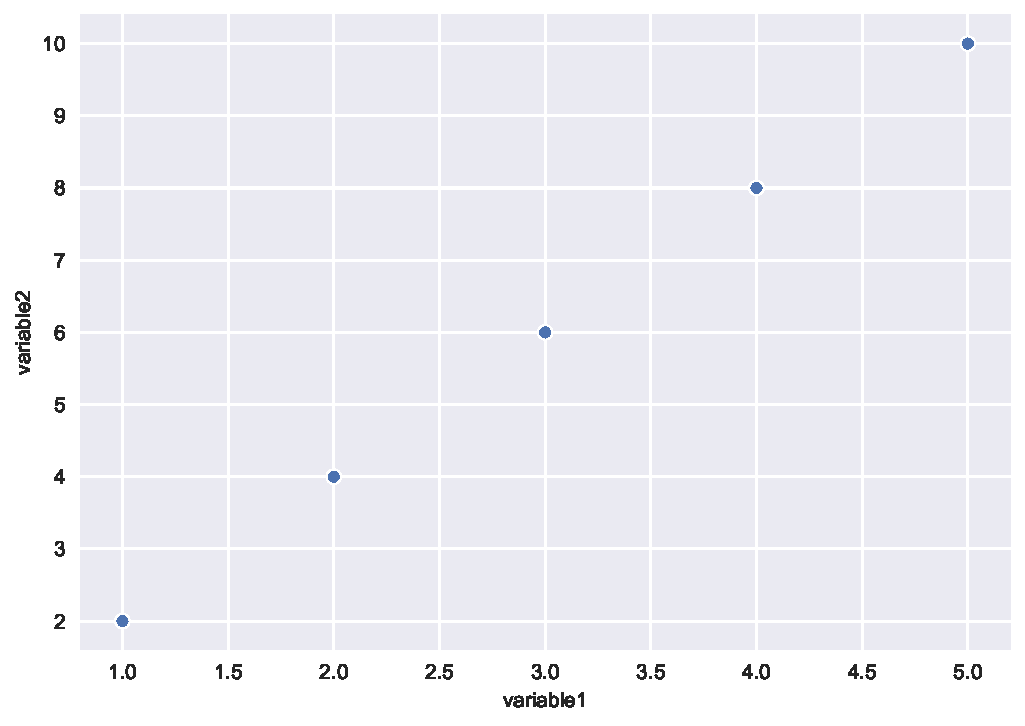
\includegraphics{index_files/figure-pdf/cell-28-output-1.pdf}

}

\end{figure}

En este ejemplo, cargamos nuestros datos y utilizamos la función
\texttt{scatterplot()} de Seaborn para crear el gráfico de correlación.
Simplemente especificamos las variables que queremos comparar en los
ejes x e y.

\hypertarget{mejores-pruxe1cticas-y-consejos}{%
\section{Mejores prácticas y
consejos}\label{mejores-pruxe1cticas-y-consejos}}

Cuando se trata de crear gráficos efectivos en Python, es importante
seguir algunas mejores prácticas que aseguren la organización, claridad
y legibilidad de tus visualizaciones. Aquí te presentamos algunos
consejos útiles:

\hypertarget{organizaciuxf3n-y-estructura-de-los-gruxe1ficos}{%
\subsection{Organización y estructura de los
gráficos}\label{organizaciuxf3n-y-estructura-de-los-gruxe1ficos}}

\begin{itemize}
\tightlist
\item
  Utiliza títulos claros y descriptivos para tus gráficos.
\item
  Etiqueta correctamente los ejes x e y para indicar qué representan.
\item
  Agrega leyendas y anotaciones para proporcionar información adicional
  sobre los elementos del gráfico.
\item
  Considera la inclusión de una clave de color si tienes múltiples
  categorías o variables.
\end{itemize}

\hypertarget{selecciuxf3n-adecuada-de-gruxe1ficos-seguxfan-los-datos}{%
\subsection{Selección adecuada de gráficos según los
datos}\label{selecciuxf3n-adecuada-de-gruxe1ficos-seguxfan-los-datos}}

\begin{itemize}
\tightlist
\item
  Elige el tipo de gráfico adecuado para representar tus datos. Algunos
  ejemplos comunes incluyen gráficos de línea, barras, dispersión y
  pastel.
\item
  Considera las características y propiedades de tus datos, como el tipo
  de variable (categórica o numérica) y la distribución, al seleccionar
  el gráfico más apropiado.
\end{itemize}

\hypertarget{optimizaciuxf3n-de-la-legibilidad-y-claridad}{%
\subsection{Optimización de la legibilidad y
claridad}\label{optimizaciuxf3n-de-la-legibilidad-y-claridad}}

\begin{itemize}
\tightlist
\item
  Asegúrate de que el tamaño del gráfico sea adecuado para su
  visualización, evitando que los elementos se superpongan o se vuelvan
  ilegibles.
\item
  Utiliza colores y estilos que sean fáciles de distinguir y que
  resalten la información importante.
\item
  Evita el exceso de elementos decorativos que puedan distraer la
  atención del mensaje principal del gráfico.
\end{itemize}

\hypertarget{bibliotecas-populares-para-gruxe1ficos-en-python}{%
\section{Bibliotecas populares para gráficos en
Python}\label{bibliotecas-populares-para-gruxe1ficos-en-python}}

Afortunadamente, Python cuenta con varias bibliotecas populares que
facilitan la creación de gráficos de calidad. Aquí te presentamos
algunas de las más utilizadas:

\hypertarget{matplotlib-1}{%
\subsection{Matplotlib}\label{matplotlib-1}}

Matplotlib es una biblioteca ampliamente utilizada y flexible que
proporciona una gran variedad de funciones y estilos para crear gráficos
estáticos. Es una excelente opción para aquellos que desean un control
detallado sobre la apariencia de sus visualizaciones.

\hypertarget{seaborn}{%
\subsection{Seaborn}\label{seaborn}}

Seaborn es una biblioteca basada en Matplotlib que simplifica la
creación de gráficos estéticamente agradables. Ofrece una interfaz de
alto nivel y opciones predefinidas para la visualización de datos
estadísticos y de análisis exploratorio.

\hypertarget{plotly}{%
\subsection{Plotly}\label{plotly}}

Plotly es una biblioteca interactiva que permite crear gráficos
interactivos y dinámicos, incluyendo gráficos en 3D, diagramas de
dispersión animados y mapas interactivos. Además, ofrece opciones de
visualización en la web y la posibilidad de compartir tus gráficos en
línea.

\hypertarget{bokeh-1}{%
\subsection{Bokeh}\label{bokeh-1}}

Bokeh es otra biblioteca de visualización interactiva que se centra en
la creación de gráficos interactivos de alta calidad para la web. Ofrece
una sintaxis sencilla y la posibilidad de crear gráficos interactivos
con herramientas de zoom, selección y desplazamiento.

\hypertarget{casos-de-estudio-y-ejemplos-pruxe1cticos}{%
\section{Casos de estudio y ejemplos
prácticos}\label{casos-de-estudio-y-ejemplos-pruxe1cticos}}

La visualización de datos con Python no solo es útil en teoría, sino que
también puede aplicarse en diversos casos de estudio y ejemplos
prácticos. Veamos algunos ejemplos interesantes:

\hypertarget{visualizaciuxf3n-de-datos-de-ventas}{%
\subsection{Visualización de datos de
ventas}\label{visualizaciuxf3n-de-datos-de-ventas}}

Imagina que eres el gerente de ventas de una empresa y quieres analizar
el rendimiento de tus productos en diferentes regiones. Utilizando
gráficos de barras y gráficos de dispersión, puedes representar
visualmente las ventas por región, identificar patrones de crecimiento y
comparar el desempeño de productos específicos. Estos gráficos te
ayudarán a tomar decisiones informadas para mejorar tus estrategias de
ventas.

\hypertarget{anuxe1lisis-de-sentimientos-en-redes-sociales}{%
\subsection{Análisis de sentimientos en redes
sociales}\label{anuxe1lisis-de-sentimientos-en-redes-sociales}}

Las redes sociales son una fuente inagotable de datos. Si estás
interesado en analizar el sentimiento de los usuarios hacia una marca o
un evento específico, puedes utilizar técnicas de procesamiento de
lenguaje natural y visualización de datos para mostrar la distribución
de sentimientos en forma de gráficos de barras, gráficos de tarta o
gráficos de líneas. Esto te permitirá comprender mejor la percepción de
los usuarios y tomar medidas adecuadas en función de los resultados
obtenidos.

\hypertarget{gruxe1ficos-interactivos-para-anuxe1lisis-financiero}{%
\subsection{Gráficos interactivos para análisis
financiero}\label{gruxe1ficos-interactivos-para-anuxe1lisis-financiero}}

En el ámbito financiero, es crucial comprender y analizar datos
complejos de manera interactiva. Puedes utilizar bibliotecas como Plotly
o Bokeh para crear gráficos interactivos que te permitan explorar datos
financieros en tiempo real, aplicar filtros, realizar zoom y obtener
detalles específicos sobre puntos de datos. Estos gráficos interactivos
facilitan el análisis financiero y te ayudan a tomar decisiones más
fundamentadas en tus inversiones.

Estos casos de estudio y ejemplos prácticos son solo algunas de las
muchas aplicaciones de la visualización de datos con Python. Desde el
análisis de ventas hasta el monitoreo de sentimientos en redes sociales
y el análisis financiero, las posibilidades son infinitas. ¡Explora,
experimenta y descubre cómo la visualización de datos puede potenciar tu
análisis y comprensión de la información!

\hypertarget{recursos-adicionales-y-pruxf3ximos-pasos}{%
\section{Recursos adicionales y próximos
pasos}\label{recursos-adicionales-y-pruxf3ximos-pasos}}

La visualización de datos con Python es un campo amplio y emocionante, y
hay muchos recursos disponibles para seguir aprendiendo y perfeccionando
tus habilidades. Aquí tienes algunos recursos adicionales que te pueden
ser útiles:

\hypertarget{enlaces-a-tutoriales-y-documentaciuxf3n}{%
\subsection{Enlaces a tutoriales y
documentación}\label{enlaces-a-tutoriales-y-documentaciuxf3n}}

\begin{itemize}
\item
  \textbf{Documentación oficial de Matplotlib}: La documentación oficial
  de Matplotlib es una fuente completa de información sobre la
  biblioteca. Puedes encontrar tutoriales, ejemplos de código y una guía
  detallada para aprovechar al máximo todas las funcionalidades que
  ofrece.
\item
  \textbf{Documentación oficial de Seaborn}: Si estás interesado en
  explorar más sobre Seaborn, la documentación oficial es un recurso
  invaluable. Aquí encontrarás ejemplos de gráficos, descripciones de
  las funciones y consejos para crear visualizaciones atractivas.
\item
  \textbf{Documentación oficial de Plotly}: Para aquellos que deseen
  adentrarse en la visualización de datos interactiva, Plotly ofrece una
  documentación detallada. Aprende cómo crear gráficos interactivos,
  agregar animaciones y personalizar tus visualizaciones.
\end{itemize}

\hypertarget{otras-fuentes-de-aprendizaje-y-comunidad}{%
\subsection{Otras fuentes de aprendizaje y
comunidad}\label{otras-fuentes-de-aprendizaje-y-comunidad}}

\begin{itemize}
\item
  \textbf{Cursos en línea}: Existen plataformas en línea que ofrecen
  cursos especializados en visualización de datos con Python. Algunos
  sitios populares incluyen Coursera, Udemy y DataCamp. Estos cursos te
  brindarán una base sólida y te guiarán a través de ejemplos prácticos.
\item
  \textbf{Foros y comunidades}: Únete a comunidades en línea dedicadas a
  la visualización de datos, como el subreddit r/dataisbeautiful o los
  grupos de LinkedIn especializados. Estos espacios te permitirán
  conectarte con otros entusiastas de la visualización de datos, hacer
  preguntas y obtener consejos valiosos.
\item
  \textbf{Libros y recursos impresos}: Explora libros dedicados a la
  visualización de datos en Python, como ``Python for Data Analysis'' de
  Wes McKinney o ``Python Data Science Handbook'' de Jake VanderPlas.
  Estos recursos ofrecen una visión más detallada y práctica de la
  visualización de datos.
\end{itemize}

¡Recuerda que la práctica constante es clave para mejorar tus
habilidades en la visualización de datos! No dudes en experimentar con
diferentes conjuntos de datos, probar nuevas técnicas y explorar las
posibilidades que Python ofrece en este campo.

En este blog, hemos cubierto una amplia gama de temas relacionados con
la visualización de datos en Python. Espero que hayas encontrado
información útil y te sientas inspirado para explorar y crear
visualizaciones impactantes. ¡No dudes en compartir tus creaciones y
experiencias con la comunidad!

Si tienes alguna pregunta o necesitas más recursos, ¡no dudes en
comunicarte! ¡Feliz visualización de datos!


\printbibliography


\end{document}
